%HEVEA \def \footertext {}
\documentclass[a4paper]{book}
\usepackage{fullpage}
\usepackage{color}
\usepackage{array}
\usepackage[utf8]{inputenc}
\usepackage[T1]{fontenc}
\usepackage[unicode]{hyperref}
% \usepackage[frenchb]{babel}
\usepackage{times}
\usepackage{courier}
\usepackage{helvet}
\usepackage{alltt}
\usepackage{graphicx}
\usepackage{xspace}
\usepackage{ifthen}
% \usepackage{floatflt}
\usepackage{verbatim}
\newcommand{\matosrevision}{2282}
			\newcommand{\matosversion}{Fig}
		

\newcommand{\sbs}[1]{\(\mbox{}_{#1}\)}
\newcommand{\ordre}{\sqsubseteq}
\newcommand{\labels}{\mathbf{Lab}}

\newcommand{\class}[1]{\textbf{\textsf{#1}}}
\newcommand{\package}[1]{\textit{\textsf{#1}}}
\newcommand{\method}[1]{\textsf{#1}}
\newcommand{\ma}{Mobile Applications Analyser\xspace}
\newcommand{\Gallery}{true}

%TODO: MAJ toutes les references Hevea!


%HEVEA \title{Matos - Manuel de l'administrateur - Version \matosversion}
%HEVEA \author{France Telecom - R\&D - MAPS/AMS}
%HEVEA \maketitle

\begin{document}
\begin{titlepage}
\begin{center}

\begin{tabular}{p{211pt}p{211pt}}

\includegraphics[width=20mm]{figures/orange} &
\begin{minipage}[b]{200pt} 
\begin{flushright}
\textbf{\large France Telecom} \\
\textbf{\large Research \& Development} \\
\textbf{MAPS}\\[0.5cm]
\mbox{}
\end{flushright}
\end{minipage}
\end{tabular}

%\the\textwidth

\huge

\vfill 

\textbf{\textsf{User's Guide to the}} \\ 
\textbf{{\textsf{MOBILE APPLICATIONS ANALYSER}}} \\ 
\vspace{1cm}
\Large
\textsf{Version \matosversion}\\
\textsf{Revision \matosrevision}\\
\vspace{1cm}

\vfill

\end{center}

\vfill 

December 2010

\end{titlepage} 

%===========================================================================
\chapter*{Preface}

\section*{Legal Notice}
The \ma was designed and developed at France
Telecom Research \& Development. Copyright (C) France Telecom
2004-2012. Any reproduction or reuse of all or part of the content of
this software (including documentation) in any form or using any media 
is strictly prohibited. Failure to respect these terms shall be considered a
breach of intellectual property and may be punishable by law.

The \ma makes use of the following libraries or software:
\begin{itemize}
\item Soot 2.3 - Copyright Sable Group, Mc Gill University, Montreal -
GNU Library General Public License. 
\item NSIS - Copyright (C) 1999-2003 NullSoft, Inc (Zlib licence).
\item BCEL 5.2 - Copyright (C) Apache Software Foundation - Apache License 2.0
\item POI - Copyright (C) 2002-2003 Apache Software Foundation - Apache License
2.0
\item JFreeChart - Copyright (C) 1991-1999 Free Software Foundation, Inc -
GNU Lesser General Public License.
\item Sqlite-jdbc - Copyright (C) 2007-2012 Taro L. Saito - Apache License 2.0
\item commons-io, commons-fileupload, commons-lang - Copyright (C) Apache Software Foundation - Apache License 2.0
\end{itemize}

\section*{Typographic Conventions}
The following typographic conventions are used in this manual:
\begin{itemize}
\item The first time an important term is introduced, it is presented
  in \emph{italics}.
\item Commands, file names and paths, and Java functions, are presented in \texttt{fixed font}.
\end{itemize}

\section*{System Requirements} \label{SysReqs} 
\ma runs under Windows XP and Linux systems (tested under a Mandriva
distribution) and requires a Java Runtime Environment 1.6 (tested with Sun JRE).
%(versions 1.3.1 up to 1.5.0).

\section*{Contact the Support Team!}
Feel free to contact us for any information or trouble using the
\ma.
\begin{itemize}
\item E-mail: \texttt{\textbf{matosteam@orange-ftgroup.com}}
\end{itemize}


%===========================================================================
\tableofcontents
%===========================================================================
\chapter*{Introduction}
\addcontentsline{toc}{chapter}{Introduction}


France Telecom's \ma is a framework to perform various analyses
on Android applications or MIDlet suite. 
Its main purpose is to check that mobile applications conform to a well
defined \emph{security policy}. Typically, a security policy may forbid the application to send short messages (SMS), open datagram or HTTP connections, or read a given system property. The \ma verifies whether the mobile application makes use (and how) of a  set of given
features. This is the purpose of the main phase of the overall
\emph{analysis process}, introduced as Features Usage phase below.
To achieve this, the \ma works on the main files that make up an
application: for example, for a MIDlet, the JAR, which contains the application
executable code, and the JAD, which is a readable descriptor of the application.

Though the analysis process is partly hard-coded in the tool, the \ma
is mainly guided by an \emph{analysis profile}, a document that
describes what is to be checked on the application. The analysis profile basically
defines the instructions to give to the \ma. 
There are mainly two kinds: what is to be observed, and
what reaction must be taken (in particular, what to report, pass or
fail, etc.) according to the observations done. 
When launching the analysis process, the user must specify which profile is
used for this analysis.

The analysis process is a sequence of \emph{phases} applied one after
another on the target application, each phase being specialized in a
specific treatment.

Currently, three phases are defined:
\begin{description}
  \item[The Class Identification phase:] that isolates midlets and checks that
  some system class are not reimplemented by the application and isolates some
  specific objects (as Views in Android).
  \item[The Descriptor Conformity phase:] checks the correctness of descriptors, namely 
  the JAD file, and the manifest file located into the JAR. This phase is
  applied at the level of the MIDlet suite. For Android applications, this phase
  extract some relevant information from the Android Manifest.
  \item[The Features Usage phase:] checks the way some
  well-identified Java features are used by the MIDlet(s) of the JAR or the
  components of the DEX file, by analysing what values can be taken by their
  arguments during all possible executions of the application. 
  This phase is applied to each MIDlet contained in the MIDlet suite but it is
  usually global for the components of the android application.
\end{description}

A \emph{MIDlet suite} is a Java application using the MIDP platform (with J2ME
CLDC configuration). It is composed of individual component (often only one)
called \emph{MIDlets}. An android application is made of different components
(namely activities, services, content providers and broadcast receivers) defined
in a single package known as the APK file (Android package). The APK file
contains an Android Manifest that is the equivalent of the JAD file, some
arbitrary resources and a code file known as the DEX file. It corresponds to the
JAR file.
%%% Local Variables: 
%%% mode: latex
%%% TeX-master: "Users-manual"
%%% End: 

%===========================================================================
\chapter{Installation}


Make sure you have a Java Runtime Environment installed first
(cf. System Requirements, page \pageref{SysReqs}).

\section{Windows Version}
Run the \texttt{setup.exe} file provided in your \ma distribution. The
installer works as a very classical Windows application installer,
just keep all default settings and press \texttt{Next} twice then
\texttt{Install}. A more detailed explanation follows:
\begin{itemize}
\item The first screen lets you select if you want to install the menu shortcuts in the main Startup menu. The answer is usually yes
\item The second screen lets you select the default destination folder. Consider the next warning if you are not using Windows XP
%\item The third screen lets you define a folder where the results of your
analysis will be stored. By default it is in the matos folder.
\item The last screen installs the tool. The complete installation requires around 5Mbytes.
\item An ``uninstaller'' is provided with the tool.
\end{itemize}

Warning: we cannot guarantee that this software is compatible with either
Windows Vista or Windows 7. Nevetheless, it is written as a pure Java
application and should work on those newer operating systems.

%\paragraph{Warning if you are not using XP} 
% \begin{itemize}
% \item Space characters in paths are badly handled. So, you must install the
%   \ma at the root level of the C: volume for example, rather than in
%   the traditional \texttt{Program Files} directory.
% \item The \texttt{matos.wsf} script is the one used to
% start the tool in interactive mode. This launcher makes use of the
% VBScript language, for which Windows XP has a built-in interpretor;
% for the NT4 version however, install the scripting languages package from
% Microsoft called \emph{Windows Script}. Check-out
% http://www.microsoft.com/downloads. The file you need is known as 
% \texttt{scr56en.exe}. 
% \end{itemize}

\subsection*{Warning about changes in your Java configuration}
If you install the \ma \emph{then later} change the installation directory
of your Java environment, the \ma won't find the new place by itself. It is
necessary to update the \texttt{matos.bat} launch script accordingly; this update
can be done automatically by executing the \texttt{initlauncher.wsf} script.

\section{Linux Version}
The software is provided as a kind of configurable and self-extractable archive
implemented as a shell-script. Open a terminal window and launch the
\texttt{./linux-installer} command in the directory where you put it.

The installer will perform the following step:
\begin{itemize}
\item it checks if all the shell commands it needs are available
\item it tries to find a java executable on your machine using simple 
heuristics
\item it proposes paths for the executable and the \ma library
\item it installs the software itself
\item it offers the possibility to configure a work repository where all the
results of analysis will be stored.
\end{itemize}

The installer tries to guess reasonable values for the installation paths. Just
type return if they are correct, otherwise, type in the right value.

Depending on whether you are logged as the super-user (root) or not, the 
installer will attempt a multi-user or a single user installation and
change the default settings.

The installation process has been tested on Mandrake/Mandriva and RedHat 
distributions. It relies on fairly standard tools and should work on 
other Linux distributions. Contact the support
team if you encounter any problem during the installation phase.

Make sure the \texttt{bin} folder of your installation directory
is included in your \texttt{PATH} environment variable, so that the
main command \texttt{matos} can be found.

\section{Adding Your License File} \label{AddingLicenseYourFile}

When you purchased the \ma, you received a license file. All you need to do
is to copy that file to the \texttt{license} folder that you'll find
in your installation directory on Windows (\texttt{lib/matos/license}
folder on Linux). To avoid problems when you update your version of the \ma, we
recommend that you keep a copy of that file in a safe place and never modify it. Contact the support
team if you encounter any problem related to the license.

\ifthenelse{\equal{\Gallery}{true}}{
\section{Creating database} \label{CreatingDatabase}
\textbf{If you do not plan to use this feature, please skip this section.}

There are different modes of operations of the \ma. In some of them, it is
useful to back-up your results in a real database. 
The \ma tool is able to use a SQL database to store CID files and to
manage the results  of analysis that have been performed on MIDlets.


The installation procedure is specific to the kind of database that will be used. 
We give here an example of a such installation for a MySQL \footnote{Although
the SQL commands issued by Coverity are pure standard SQL commands, we
recommend to use this database engine.} database, on a Windows system:

\begin{itemize}
  \item First, you need to install the database management system itself (if it
  is not already installed on the computer). An easy way to do so is to download
  and install EasyPHP (http://www.easyphp.org/).

  \item Second, you need to create the database, a user and the necessary
  tables that the \ma will use. To launch the database administration tool,
  rigth click on EasyPHP's tray icon and choose 'Administration', then click on 
  the 'Manage Database' link, and then click on the SQL icon on the left frame
  to open a query window. 
%  Click on 'Import file' and browse to select the file named
%  \texttt{initdb.sql} that comes with the installation files and click on 'Go'.  
  Select the 'mysql' database, copy paste the following mysql script into the text area and click on 'Go'
\end{itemize}
  \verbatiminput{initdb.txt} 

  By default, the database can only be accessed by the local computer.
  If you want it to be accessible from other computers, you have to:
  	\begin{itemize}
	    \item Set a root password (for security reasons):
		\begin{itemize}
			\item Launch the phpMyAdmin (rigth click on EasyPHP's tray icon and choose
			'Administration') and click on 'Manage Database' then on 'Privileges' and
			edit privileges of the root user. Set the password and click on the 'Go' 
			button.
			\item Edit the C:$\backslash$Program Files$\backslash$EasyPHP1.8$\backslash$phpmyadmin$\backslash$config.inc.php and
			put the new password for the root user:
			\newline \texttt{\$cfg['Servers'][\$i]['user'] = 'root';}
 			\newline \texttt{\$cfg['Servers'][\$i]['password'] ='the-new-password-4-root';} 
 			\newline Save the file.
	    \end{itemize}
	    \item Configure the database to allow distant access:
	    Rigth click on EasyPHP's tray icon and choose the menu entry
	    \texttt{Configuration->MySQL} to open the \texttt{my.ini} configuration
	    file and add a semi column (;) before the line defining the binding address
	    to comment it out:\newline
	    \texttt{bind-address=127.0.0.1} 
	    \newline Save the file.
	\end{itemize}

Use the following parameters to configure the \ma tool to connect to this
newly created database (using menu Tools->Databse Management
Tool->Edit->Database properties\ldots):
  	\begin{itemize}
        \item \texttt{\textbf{matos.dbUrl=jdbc:mysql://localhost/matos}} ,
        \item \texttt{\textbf{matos.dbLogin=matos\_user}} ,
	    \item \texttt{\textbf{matos.dbPasswd=matosPassword}} 
    \end{itemize}

}{}
%%% Local Variables: 
%%% mode: latex
%%% TeX-master: "Users-manual"
%%% End: 

%===========================================================================
 \chapter{Getting Started}
%TODO: Incomplet, ``l'exercice'' propos� en fin de chapitre est ridiculement restreint pour l'instant.

 There are several usage scenario for the \ma. We present here the interactive
 use of the tool. The goal of this chapter is to get you familiar with the \ma's
 interface in half an hour. We assume you have already installed the tool .

 \section{Launching the \ma}
 First ensure that you have copied your personal license file to the
 \texttt{license} folder (cf. \S \ref{AddingLicenseYourFile}). Launch the
 \ma with \texttt{Start -> Programs -> Midlet Analyser -> Start}
 on Windows, or by typing \texttt{matos} in a Linux shell. The
 window shown on figure \ref{figGUIMainWin} appears. 
 
\ifthenelse{\equal{\Gallery}{true}}{ 
 \begin{figure}[h]
 \begin{center}
 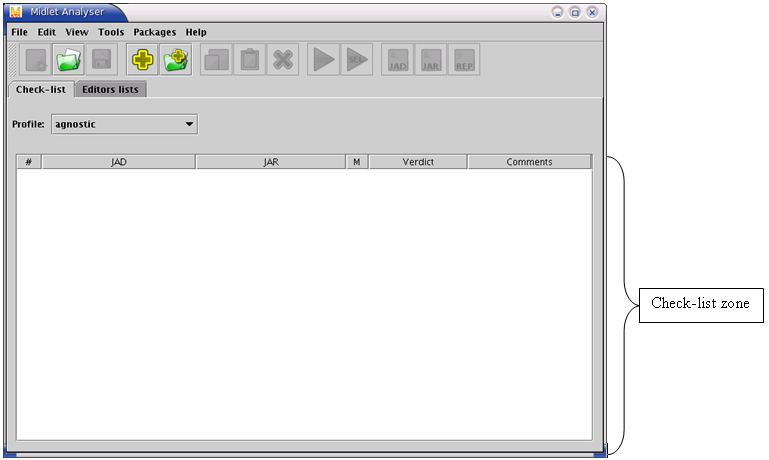
\includegraphics[width=14cm]{figures/GUI-main-Gallery}
 \end{center}
 \caption{Graphical user interface, main window}
 \label{figGUIMainWin}
 \end{figure}
}{
 \begin{figure}[h]
 \begin{center}
 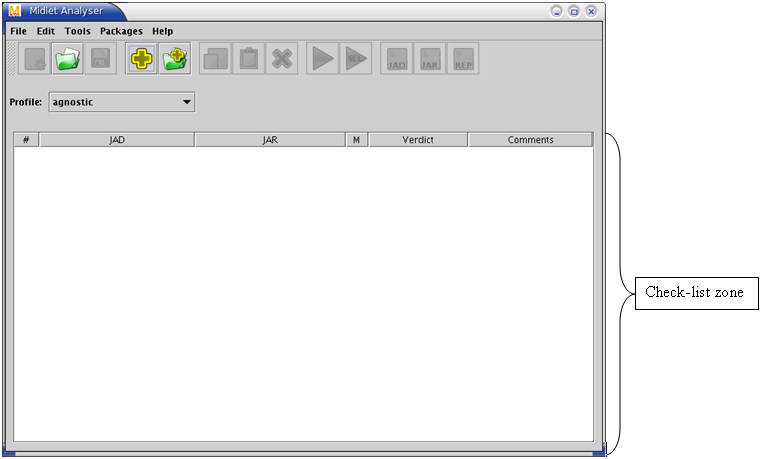
\includegraphics[width=14cm]{figures/figures/GUI-main-OP}
 \end{center}
 \caption{Graphical user interface, main window}
 \label{figGUIMainWin}
 \end{figure}
}

 \subsection*{The check-list zone}
 The main part of the interface is called the \emph{check-list} zone. It is a table
 representing what analyses are going to be performed when you start
 the process. An analysis, represented by a single row in the
 table, is also called a \emph{check-step}. It is one step among all the steps
 of the sequence.
 \subsection*{Keep music in mind!} 
 The concept of check-list is very similar to the concept of \textbf{play-list}
 in an audio player such as Windows Media Player\texttrademark. In an
 audio player, you define a list of songs you want the tool to
 play back: you can add songs from your hard disk to the play-list (one
 by one or a whole directory), remove some from the list, maybe change
 some properties (MP3 tags?) of the songs, then finally PLAY the whole
 list. You can even save the play-list you've defined if you like it,
 so you can replay it exactly the same way tomorrow.  

 In the \ma, you manage check-lists instead of play-lists. You define
 a list of analyses you want the tool to execute. You can add an analysis
 for a MIDlet file located on your hard disk or on the Web, add an
 analysis for each MIDlet file of a directory, remove analyses from the
 check-list, change some properties of analyses, then ``PLAY'' the global
 analysis process. In the \ma too you can save and load back your
 check-lists.


 \section{Checking a MIDlet suite}

Let's analyse a single JAR file. In chapter \ref{BasicUsage}, you will find how to analyse a series of
files, and more.

 \begin{figure}[h]
 \begin{center}
 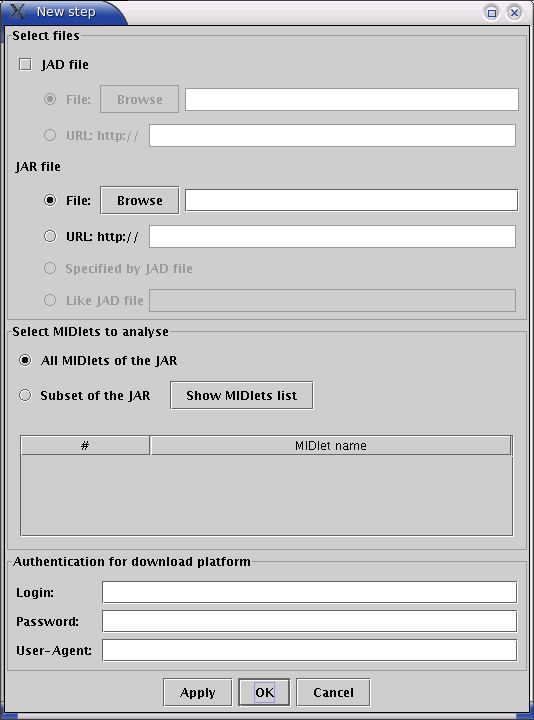
\includegraphics[width=10cm]{figures/GUI-new-step-dialog}
 \end{center}
 \caption{Adding a new check-step (one single MIDlet suite)}
 \label{figAddingMIDletSuite}
 \end{figure} 

 \begin{figure}[h]
 \begin{center}
 
\includegraphics[width=1.2cm]{figures/buttonAnalyseSelection}
 \end{center}
 \caption{Button to launch analysis of selected step}
 \label{figButAnalyse}
 \end{figure}

 \begin{figure}[h]
 \begin{center}
 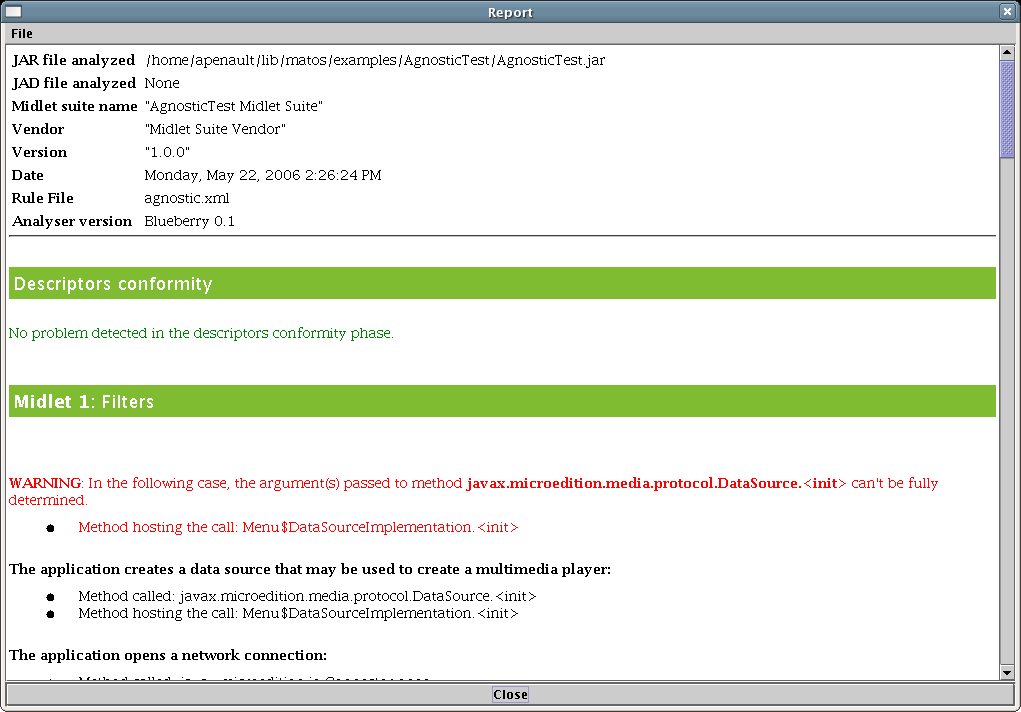
\includegraphics[width=15cm]{figures/reportAgnosticTest}
 \end{center}
 \caption{An example JAR analysis report}
 \label{figExampleReport}
 \end{figure} 
    
 \begin{enumerate}
 \item Select \texttt{File -> Add File to analyse -> Add MIDlet suite...}.
 \item The dialog shown on figure \ref{figAddingMIDletSuite} appears. 
 Since you only want to select a JAR file, ensure the \texttt{JAD file}
 option is unchecked. To specify the JAR you want, select
 \texttt{File:} in the \texttt{JAR file} zone and click
 \texttt{Browse}. Select a JAR file somewhere on your hard disk; you
 may find one in the \texttt{examples} folder of the installation
 directory, such as \texttt{AgnosticTest.jar}.
 \item Make sure the set of MIDlets to analyse is set to \texttt{All MIDlets of
 the JAR}.
 \item Click \texttt{OK}. As you can see, the check-list now contains
   one step (\#1), representing the analysis you've just
   specified. On the main window, select \texttt{agnostic} for the profile.
 \item{Click on the button shown on figure \ref{figButAnalyse} to
 analyse the selected step.} 
 \item A dialog appears, you must indicate the folder for the analysis results.
 \item When the analysis process is done, click on \texttt{Close} button. A
 window opens to show you the report. For the \texttt{AgnosticTest.jar} example
   the report window should look as shown on figure
   \ref{figExampleReport}.
 \end{enumerate}

All analysis reports are divided into three parts:
\begin{itemize}
\item The fist part until the horizontal separator identifies the MIDlet analysed and 
  summarizes the main characteristics of the analysis:
  \begin{itemize}
  \item the name of the jar file analysed
  \item the name of the jad file if one was present
  \item the name of the MIDlet suite, as registered in the manifest or in the JAD file
  \item the MIDlet vendor and the version of the suite
  \item the date of the analysis
  \item the analysis profile (rule file) used
  \item the version of the \ma
  \end{itemize}
\item the next section summarizes the error found in the
  JAD file or in the manifest such as mandatory attributes not defined
  or attributes repeated with different values.
\item the last part consists of one diagnostic section per MIDlet
  analysed. The meaning of the verdicts depends on the analysis profile
  chosen and is out of the scope of this manual. 
  
  As a \emph{convention}, PASS verdicts are written in green and FAIL verdicts are written in
  red. Warnings are written in orange and correspond to points the
  evaluator should check manually. Informative text without a priori judgement
  is written in black.
\end{itemize}

\section{Analyzing several midlets}
\subsection{Building a checklist}
\begin{figure}[h]
	\begin{center}
    	\scalebox{0.8}{
\includegraphics{figures/buttonAnalyseAll}}
   	\end{center}
   	\caption{Button to launch analysis of all steps in the current check-list}
   	\label{butAnalyseAll}
\end{figure}

\begin{itemize}
  \item Select \texttt{File -> Add directory}
  \item Select a directory with several midlets. For example
  \texttt{\${LIB}/examples/test/HttpConnection}. Three midlets should appear.
  \item Add another midlet with \texttt{File -> Add file to analyze -> Add
  MIDlet suite} and select a midlet on your hard disk.
  \item Now you have five midlets selected. You can remove one by selecting it
  and pressing the right mouse button to open the contextual menu. Then press
  remove (It removes the midlet from your check-list, not from your computer).
  \item Press the button shown on figure \ref{butAnalyseAll}.
\end{itemize}

\subsection{Saving and recovering a check-list}
\begin{itemize}
  \item Select \texttt{File -> Save as}
  \item Provide a file name for your check-list and press ``Save check-list''
  \item Now you can quit the tool and launch it again. Select \texttt{File ->
  Open} 
  \item type-in the name of your saved check-list. The elements to analyze are
   back.
\end{itemize}
\ifthenelse{\equal{\Gallery}{true}}{
\subsection{Registering and analysing an editor's list}
\textbf{This section is only relevant in the context of the Gallery portal.}
% \vspace{0.5cm}
% \begin{tabbing}
%  \hspace{0.4cm} \= 1. \hspace{1pt} \= Select \texttt{File -> Register} an editor's list.\\\\
%  \> 2. \> Select an editor's list (an Excel file) somewhere on your hard disk. A
%  row appears on the table in the \\ \> \> \texttt{Editors lists} tab.\\\\
%  \> 3. \> Select the added row and click on the \texttt{Add to check-list}
%  button. All JAR and JAD files described in \\ \> \> the editor's list are added
%  in the current check-list.\\\\
%  \> 4. \> To analyse all steps of the current check-list, click on the button
%  shown on figure \ref{butAnalyseAll}.
% \end{tabbing}
\begin{itemize}
 \item Select \texttt{File -> Register an editor's list\ldots}
 \item Select an editor's list (an Excel file) somewhere on your hard disk. A
 row appears on the table in the \texttt{Editors lists} tab.
 \item Select the added row and click on the \texttt{Add to check-list}
 button. All JAR and JAD files described in the editor's list are added
 in the current check-list.
 \item To analyse all steps of the current check-list, click on the button
 shown on figure \ref{butAnalyseAll}.
\end{itemize}
}{}


%% POSTPONED
%% \paragraph{Exercise B}
%%  %TODO
%%  [scenario2 : add a JAD [HTTP address], analyse all, popup/view report,
%%  close it.]

%%  \paragraph{Exercise C}
%%  %TODO
%%  [scenario3 : add directory, remove les 2 doublons, force a profile for
%%  all, save as, analyse all, remove all, open the saved one.]

\section{The Command Line Mode} \label{CmdLineMode}
The \ma can be used to some extent in command line mode. The main
command is called \texttt{matos}. The general syntax is:
\begin{alltt}
matos \emph{[options] [parameter]} 
\end{alltt}

When only one pararmeter is present and it is a JAR or JAD file, the tool
is launched in interactive mode. 
The GUI will open and get prepared for the analysis of the specified file (it
is added to the check-list zone). Refer to  \ref{IdentTargetFiles} to see what
happens if the parameter is a JAD file.

When at least one option is specified, the GUI won't open, and the
tool will execute fully as a batch shell command.

\subsection{Options}

\newcommand{\OptArg}[2]{\textsf{#1~\textit{#2}}}
\newcommand{\Opt}[1]{\textsf{#1}\xspace}
\newcommand{\File}[1]{\textit{#1}\xspace}
\begin{description}
%\item[\OptArg{-t }{transfile}]\setlength{\itemsep}{0cm}

\item[\OptArg{-jar }{jar-file-name}] Force the target JAR file. When
  this option is used while a JAD file is specified (using the parameter or \texttt{-jad}), the JAR URL
  specified into the JAD file is ignored. This option may also be used
  if the wanted JAR file does not carry the standard \texttt{.jar}
  extension.  This option is ignored when \texttt{-c} is used.

\item[\OptArg{-jad }{jad-file-name}] Force the target JAD file. May
  also be used if the wanted JAD file does not carry the standard \texttt{.jad}
  extension. This option is ignored when \texttt{-c} is used.
\item[\OptArg{-apk }{apk-file-name}] Force the target Android APK file. May
  also be used if the wanted APK file does not carry the standard \texttt{.apk}
  extension. This option is ignored when \texttt{-c} is used.
\item[\OptArg{-d }{profile-name}] Use the specified security profile. 
Valid profile names are those of XML files present in the 
\File{\emph{install-Matos}/lib/definitions} directory, without the
extension. This option is ignored when \texttt{-c} is used.

\item[\OptArg{-o }{output-file-name}] Output results to the specified
  output file. By default the output goes to a file called
  \texttt{output.html}. If \texttt{-c} is used, \texttt{-o} is assumed to be
  the output \emph{directory} where to store all results of the
  check-list execution. %TODO: c'est quoi le dir cr�� par d�faut ?

\item[\Opt{-pdf}] Export the output results in PDF format, the generated PDF
file as the same name and the same location as the file specified in the \texttt{-o}
option. If \texttt{-pdf} is used, the use of \texttt{-o} option is mandatory.

\item[\OptArg{-m }{midlet-name}] Among all the MIDlets contained in
  the target MIDlet suite, run the analysis for the specified MIDlet
  only. This option allows to specify explicitly what MIDlets should
  be analysed. By default, all MIDlets of the target JAR are
  analysed. To target explicitly more than one MIDlet, use multiple
  instances of this option. The MIDlet name must be a fully qualified
  MIDlet Identifier (packages names included, eg. \texttt{pack1.pack2.MyFirstMidlet}).
  This option is ignored when \texttt{-c} is used.

\item[\OptArg{-c }{check-list-file-name}] Run in check-list mode (also called ``campaign''). 
Execute the sequence of analyses specified in the check-list file
provided. Such files are \texttt{.mcl} files as those saved from the GUI. The
\texttt{-o} option here can be used to specify the output directory where to
produce all results files.  The following options are ignored when \texttt{-c}
is used: \texttt{-d},\texttt{-m},\texttt{-jar},\texttt{-jad},\texttt{-all}.

\item[\OptArg{-all }{dir-name}] Run the analysis on all application files found
  present in the specified directory. For midlets, all JAD files are taken first,
  for which the \ma uses the \texttt{MIDlet-Jar-URL} attribute to locate the
  corresponding JAR file. These files are analysed, then so are all JAR
  files of the specified directory that were not treated already
  (those that are not pointed to by JAD file). The \texttt{-all}
  option is ignored when \texttt{-c} is used.

\item[\OptArg{-tmp }{dir-name}] Ask the tool to use the specified directory as a
  temporary directory. Warning: the \ma may take the freedom to
  destroy this directory when not needed anymore. By default, the
  system's main temporary directory is used, stored in the \texttt{TEMP} environment variable.

\item[\OptArg{-css }{file-name}] Ask the tool to use the specified
  style sheet for the final presentation of the HTML output file. By
  default no presentation is applied. Please note that a ready-to-use style
  sheet called \texttt{style.css} is provided in the installation
  directory. The user is free to use that file with the \texttt{-css}
  option.
  
\item[\OptArg{-log }{file-name}] Put logs generated by the \ma during its
execution in the specified file. By default logs goes to a file called
  \texttt{log.txt} in the \File{\emph{install-Matos}/lib/} directory.

\item[\Opt{-apache}] Adapt the HTML output when the \ma is invoked
  through a web server. In particular, only the body of the document
  is generated, rather than a complete HTML document with enclosing
  \texttt{<html>} tags. In addition, the actual path of the analysed
  files is not shown in the header of the results report.
\item[\OptArg{-tmp }{dir-name}] change the temporary folder used to \verb!dir-name!.
\item[\Opt{-xml}] Output the result in XML format (\texttt{-o} must be used).  

\item[\Opt{-h}] Online help.

\end{description}

\subsection{Identification of target files}\label{IdentTargetFiles}
The files to be analysed are specified to the \ma by indicating a
path to them. The path is either a path which is relative to the
working directory or a classical HTTP URL starting with \texttt{http://}.

If the only file specified is a JAD file, the corresponding JAR
will be searched at the location specified by the 
\texttt{MIDlet-Jar-URL} attribute, in the JAD. If that attribute is
not a well-formed HTTP URL, \emph{while} the specified JAD path is
an HTTP URL, then the JAR file will be searched at the same location
as the JAD. For example, if the option
\texttt{-jad "http://www.supermidlets.com/fun/pingpong.jad"} is
specified, while the JAD contains the attribute
\texttt{MIDlet-Jar-URL: pingpong.jar}, then the tool will assume the JAR
file address is actually
\texttt{http://www.supermidlets.com/fun/pingpong.jar}.

This remark applies however the target file(s) was specified (main argument of the textual command, -jad or -jar flags, or
the \texttt{jar} or \texttt{jad} attributes in the check-list file, when
run in check-list mode).

\subsection{Examples}

\begin{itemize}
\item{\texttt{matos}}\\ 
Starts the \ma in interactive mode. The GUI is opened, with no focus
on a particular target file.
\item{\texttt{matos Pacman.jar}}\\
Starts the \ma in interactive mode. The GUI is opened in MIDP mode, with focus
on the Pacman.jar file. That file is added to the current check-list.
\item{\texttt{matos Pacman.apk}}\\
Starts the \ma in interactive mode. The GUI is opened in Android mode, with
focus on the Pacman.apk file which is an Android application. 
That file is added to the current check-list.
\item{\texttt{matos -jar Pacman.jar}}\\
Launches directly the analysis of Pacman.jar. The GUI is not opened. Since nothing more is
specified, the analysis profile used will be the one set as default in
the tool configuration. 
\item{\texttt{matos -jar Pacman.jar -o PacmanResults.html -d
    agnostic}}\\
Launches directly the analysis of Pacman.jar, using the Agnostic
security profile. The GUI is not opened. Reporting is produced in the PacmanResults.html
file.
\item{\texttt{matos -jad Pacman.jad}}\\
Only the JAD is provided here: the tool will search for its associated
JAR at the location indicated by the \texttt{MIDlet-Jar-URL} attribute
of the JAD.
\end{itemize}

%%% Local Variables: 
%%% mode: latex
%%% TeX-master: "Users-manual"
%%% End: 

%===========================================================================
\chapter{The Analysis Process}

For each MIDlet suite, the \textbf{analysis process} consists of the
sequential execution of phases. Each phase is dedicated to the control
of particular characteristics, and its scope is either global
(the analysis target is the entire MIDlet suite) or local (per MIDlet
analysis). In that sense, in its simplest use the \ma should be seen as a
\textbf{sequencer of phases} over a given MIDlet suite. This is
illustrated in figure \ref{figSAA}, where analysis parameters are at least a JAR
file and a profile.


\begin{figure}[h] 
\begin{center}
\scalebox{0.6}{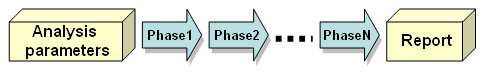
\includegraphics{figures/Sequencer1D}}
\end{center}
\caption{A single analysis process execution}
\label{figSAA}
\end{figure}

\begin{figure}[t]
\begin{center}
\scalebox{0.58}{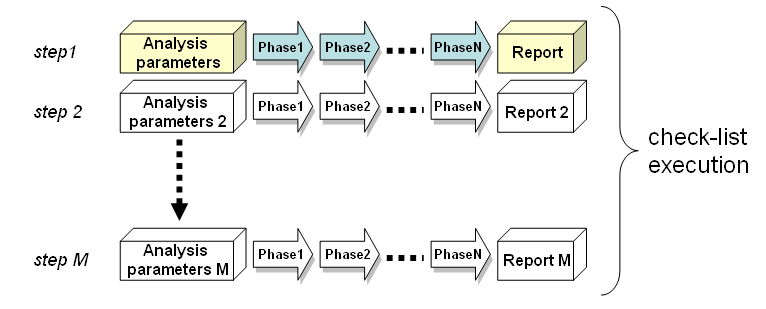
\includegraphics{figures/Sequencer2D}}
\end{center}
\caption{A check-list execution}
\label{figSeq2D}
\end{figure}


So far, only three phases are available but we plan to add new ones in
a future release of the tool. Besides, note that executing a
check-list means to run the analysis process several times
in sequence, as shown on figure \ref{figSeq2D}.


\section{The Descriptors Conformity Phase (MIDP)}
The Descriptors Conformity phase checks the wellformed-ness and completeness of the
descriptors that can be associated with a MIDlet suite: 

\begin{itemize}
\item the JAD file (optional)
\item the JAR manifest file (mandatory), which contains similar information to the
  JAD's.
\end{itemize}

Some rules apply all the time, while others apply only if
the two files are present since they are related to their mutual
consistency (remember the presence of a JAD is optional). The main
problems that can be reported are listed below.


\subsection{Problems that may happen in any descriptor (JAD or
  Manifest)}
\begin{itemize}
\item Mandatory attribute missing
\item Incorrect value for an attribute
\item Double definition of an attribute
\item MIDlet declaration is malformed. Three parameters (name, icon,
  class name) are expected; however the icon parameter may be empty.
\item Name for a MIDlet missing
\item Class name for a MIDlet missing
\item Class for a MIDlet declared in the descriptor actually does not exist
  in the JAR file
\item Icon for a MIDlet declared in the descriptor actually does not exist
  in the JAR file
\item Icon for a MIDlet declared in the descriptor actually does not seem to
  be a PNG file 
\end{itemize}

\subsection{Problems specific to the JAD}
\begin{itemize}
\item Can't read certificate \emph{n} in path (\emph{m}).
\end{itemize}

\subsection{Problems that may happen if the two descriptors are provided}
\begin{itemize}
\item Mandatory attribute defined in none of the descriptors
\item The JAR file size and the value indicated in the JAD differ
\item Name for a MIDlet differs from the JAR manifest to the JAD
\item Icon for a MIDlet differs from the JAR manifest to the JAD
\item Class for a MIDlet differs from the JAR manifest to the JAD
\end{itemize}

Some of the checks can be customized. It is possible to add constraints on
midlet names, on actions and suffixes handled by CHAPI,  on URLs handled
by PushRegistry.
It is also possible to restrict the number of visible midlet and to impose
constraints on icon sizes.

% \paragraph{Remark} The descriptors conformity phase is a built-in
% phase of the \ma. As a consequence, rules above currently can't be
% customized by the user (in contrast to the Features Usage phase, which
% can be defined in an analysis profile). Another consequence is that
% the Descriptors Conformity phase is run exactly the same way whatever
% the profile used. We are considering improving that in a future
% release of the tool.

\subsection*{Customize some properties of descriptors}
The descriptors conformity phase checks the conformity of descriptors
according to MIDP 2.0 specification and JAR file specification. Nevertheless,
you can add properties in the security profile that have to be 
verified by descriptors. These properties concern:
\begin{itemize}
  \item Line end separators in the JAD file and in the JAR manifest file.
  \item Order of attributes in the descriptors.
  \item Mandatory and forbidden attributes in these files.
\end{itemize}
This customization is detailed in section \ref{CustoConform} of this document.

\section{Android Manifest}
This phase extracts some useful information from the manifest as stored in the
APK file:
\begin{itemize}
  \item The supported screen sizes and density
  \item The permissions used by the midlet (in red, Android system permissions)
  \item The features required if any 
  \item The SDK requirements if documented.
\end{itemize}
\section{The Static Analysis Phase} 
The static analysis phase was initially centered only around feature usage.  As
this phase involves the building of several complex intermediate models that 
are useful for many useful checks,  it has evolved and now contains other 
analysis not directly related to feature usage.

\subsection{The principle of feature Usage}
The \ma's main purpose is to check whether some particular Java features
are used by the MIDlet, and how. This is called the Features Usage
phase. Technically, a Java feature is one particular method of a
particular Java package. The principle is quite simple:

\begin{itemize}
\item A feature is defined by a method of the MIDP profile (or a related
JSR) and a set of arguments. Methods and their arguments  are
identified and declared in an analysis profile.
\item When you run the analysis process, the tool will look for every
  invocation of that method in the MIDlet, and gather information
  about:
\begin{itemize}
\item Where the call is located in the code.
\item The values taken by the arguments during that call, or returned
  by the call. 
\end{itemize}
\item When the process is done, a report will be produced according to
  the report directives that are specified in the analysis profile. 
\end{itemize}

So, the \ma does not only detect the use of a given feature: it can also
computes an upper approximation of the possible values of the parameters passed
to that method at runtime. 

It is important to understand the kind of approximation
handled by the tool. Matos uses three kinds of abstract values: concatenated 
strings, integers and objects.

The tool has been optimized for handling \textbf{character strings}. Basic
approximations are regular constant strings, the ``unknown object'' 
representing any string and coded as \verb!"\*"! and method calls that  have not
been resolved (when the method is not recognised by Matos) which are represented by
\verb!"\[qualified.methodName\]"!. Backslashes in constant strings are escaped
(\verb!\\!). Those objects can be directly concatenated. For example
\verb!"aa\*bb"! represents any string begining with \verb!"aa"! and ending with
\verb!"bb"!. Approximations are sets of such strings.

Arguments of type \textbf{integer} (\texttt{int}) are computable only if
they appear straight as constants in the MIDlet source code.

Class object can also be tracked if they are created as constants and not
extracted from objects. A class object is represented as the name of the class
between brackets.

Finally other kind of objects are represented by the point where they have been
``allocated''. Those points are represented by the type of object they generate
and a unique identifier (a number). They are refered in results by their number 
and written such as \textbf{[5]}.

To help you distinguish different usage of values generated by the system, this version of Matos distinguishes two kinds of allocation points. Real allocation
points defined by a new expression and fake allocation points corresponding to
the point where a CLDC/MIDP method returns a value to the application. Those
allocation are further defined by the program point where the system method was
called.

A program point is defined as a bytecode offset in a method. It is
written \texttt{offset@signature} where \texttt{signature} is the full
specification of the method.

The syntax for method signature is the following:
\begin{alltt}
\textit{signature} ::= <\textit{qualifiedClassName}:\textvisiblespace\textit{subsignature}>
\textit{subsignature} ::= \textit{type}\textvisiblespace\textit{methodName}(\textit{type},\ldots,\textit{type})
\textit{type} ::= \textit{qualifiedClassName} | void | \textit{basicType}
     |  \textit{type}[]
\end{alltt}
Note that spaces are significant. Do not add spurious spaces when you write
method signatures.

It is important to be able to distinguish the two kinds of allocation points.
Two distinct allocation points corresponding to two new expressions represent
\emph{distinct} live objects. On the other hand two distinct allocation points
where at least one is a program point may represent the same live object. It
depends on the semantics of the system method called but a lot of such methods
produce new objects each time they are called.

\subsection{A typical example}
Imagine you decide in your security policy to reject MIDlets that use
the network by opening HTTP connections. 
In MIDP, opening a connection is done through a call to the generic method
\texttt{Connector.open} method with an address parameter that specifies 
which protocol to use:
\begin{verbatim}
c = Connector.open(``http://www.blablabla.org/example.html'');
\end{verbatim}

The call is dynamically protected in that case by the \emph{Net Access} 
security function group and more specifically by the 
\verb!javax.microedition.io.Connector.http! permission.

The \ma  will locate all invocations of the \texttt{Connector.open}
method, and try to
compute all the possible values of the method's argument, which
contains the target URL. If it turns out that at least one possible
value contains the prefix \texttt{http://}, then the tool will inform
you that the MIDlet violates your policy.

In the security profile, these operations are handled by two specification:
\begin{itemize}
  \item a rule that specifies the method to look at
  \item a report that tells how to analyze the result
 \end{itemize}
The rule is the following:
 \begin{verbatim}
 <rule name="HTTP-R">
 <args class="javax.microedition.io.Connector"
       method="javax.microedition.io.Connection open(java.lang.String)"
       report="HTTP">
       <argument position="0"/>
 </args>
 </rule>
\end{verbatim}
It specifies the method by its class and subsignature and the argument to
analyze. The report to use is identified by its name.

Three kinds of results can
come out of the argument analysis, actually. We give examples below:
\begin{itemize}
\item{\textbf{Full computation}}: \texttt{https://www.blablabla.org/index.html}
\item{\textbf{Partial computation}}: \texttt{ht}\emph{*}, or
  \texttt{http://www.blablabla.org/}\emph{*}\texttt{.mp3}
\item{\textbf{Impossible computation}}: \emph{*}
\end{itemize}

where the star here (\emph{*}) represents the non-computable part of the
string. Why is it not always possible to compute the full value?
It depends on the level of complexity of the application. If too
complex operations are applied to the observed data, the \ma may fail
to understand what's going on. Another simple reason is the fact that 
data may get their value externally: if the MIDlet asks the user to 
enter the entire HTTP URL at runtime, then there is no mean to guess what the
user will type.

We will use the following report:
\begin{verbatim}
<report name="HTTP">
  <pseudoString>
  	<filter name="CAPTURED" pattern="http:.*" verdict="FAILED">
  	  HTTP connection
  	</filter>
  	<filter name="OK" pattern="[^\]*:.*" verdict="PASSED">
  	  Another kind of connection
  	</filter>
  	<filter name="NOT ANALYZED" pattern=".*" verdict="FAILED">
  	  Cannot analyze the scheme of this URL
  	</filter>
  </pseudoString>
</report>
\end{verbatim}
It specifies a sequence of filters. Each filter has a name, a verdict status and
a content printed out. It is applied when the pattern filters the approximation
string computed for the argument. Patterns are specified in POSIX syntax. Note
the use of \verb![^\]*! to capture the absence of uncomputed part in the URL
scheme. We could use smarter patterns as it is sufficient to know that the first
letter is not an 'h' but it would be of little practical use.

\subsection{Further technical details}
Generally speaking, the argument analysis is based
on a computation of the possible values that can be stored at 
different program points, taking into account all possible execution
paths of the program. The computation is actually an upper
approximation of the possible values, with the implicit and safe assumption
that when something can't be computed, then it can be \emph{anything}
at runtime. 

The analysis is a \textbf{static analysis} performed on the
application bytecode: as a result, the \ma never needs to run the
MIDlet, it just reasons about its bytecode, after having built an
abstraction of it. The underlying theory is known as abstract interpretation and
was designed by Patrick and Radhia Cousot but the real tool used here is
a pointer analysis (also known as a points-to analysis).


The main purpose of the arguments analysis is to check the values of
arguments passed to certain methods, but you can also check the return
values of methods, as well as the values taken by certain class fields.
Concretely, the target variables (methods arguments, return values, or
attributes) to be checked are specified in the analysis profile. 

\section{The limits of static analysis}
As said earlier, there are cases where the \ma cannot decide whether or not
a MIDlet satisfies a security property because it cannot analyse the arguments
of a method call. To avoid those cases, it is recommended to impose 
coding constraints to developers of MIDlets so that those limits are 
never encountered in practice.

\subsection{The notion of pseudo-constant}
The main principle is that an argument of a method call whose value creates
a security risk should be \emph{almost} constant. The definition of almost 
has been relaxed in such a way to ease the life of application developers.
We will call pseudo-constants values satisfying the necessary conditions.

A simple (simplistic) definition of a pseudo constant is the following.
A pseudo-constant is an object of type string which is either one of the following:
\begin{itemize}
\item a literal or a field declared as \verb!final static! and initialised according to its definition,
\item a static field \verb!v! of a class or an instance field of an object where the class containing it is a class of the MIDlet (and not of the MIDP profile) and where all the values \verb!c! assigned to the field (\verb!v=c!) are 
pseudo-constants.
\item a variable local to a method where all the values assigned to the 
variable are pseudo-constants
\item a parameter of a method. In that case the corresponding argument in all the calls of this method in the source code of the MIDlet must be a 
pseudo-constant,
\item a call to \verb!new String(c)! where \verb!c! is a pseudo constant.
\end{itemize}
Note that the definition of pseudo-constant is recursive: it uses the notion
of pseudo-constants. So the notion of pseudo-constant is in fact 
quite expressive.

\subsection{Extending the definition of pseudo-constants}
The previous definition is very convenient to specify what is authorized to
developers but it also forbids a lot of practical usage. It can  relaxed
a little further for the \ma:
\begin{itemize}
\item if \verb!c1! and \verb!c2! is a pseudo-constant, then so is their
concatenation defined as \verb!c1 + c2! (but you cannot use an explicit global 
string buffer to create it, because the \ma cannot check if there is not
another thread using the same buffer at the same time);
\item if all the values assigned to the element of an array are pseudo-constants, so is the value of any element of the array, but be careful ! all the uses
are merged in a single one for the analysis.
\end{itemize}

If you want to use the relaxed rules, you must be careful that the average
developer will be able to understand what is authorized and what is forbidden.

As a last warning : when programmers use a global variable with
multiple usages \footnote{for example, if a variable is used to store all the newly created strings}, note that all 
the values of this variable are coalesced into a single
usage pattern by the analysis. This means that some use case may be inferred
by the \ma that do not exist in practice. Nevertheless, this set will always
be finite and the evaluator can usually decide if there is a security
 problem or not by looking at the potential values.

\subsection{Tracking arbitrary objects}
The \ma has been designed to track string constants but it may in fact track any
kind of Java object. Abstract objects correspond to roughly allocation points in
the code. An abstract object is presented in the result has an integer between
brackets. Per se it contains no useful information. But abstract objects may
appear in multiple results. In that case, it means that an object used in a
given call \emph{may} be used in another. 

There is usually an object table dumped after the results of the different
rules. This object table contains a line per abstract object that defines its
exact class (as set at the allocation point) and gives pointers to its different
uses.

It is important to understand the difference between abstract objects that
represent sets of potential live object during a real execution and a real
object. When we see a given abstract object at two different program points, it
does not mean that all live objects abstracted by this abstract object have to
be present at both points. On the other hand, if an abstract object is not
present at a given point, it means that all the real object abstracted cannot be
present at this program point. Even with those limitations, abstract objects are
useful to figure out what kind of relations link the real objects. A simple
example is given on figure \ref{objectImage}, an intent is created with a class
object \verb:Main: it is then given to  \verb!startActivity!. Without the
tracking of the abstract object, it would have been difficult to guess
if the intent using this class did corespond to a service or an activity.

\begin{figure}
\begin{minipage}{13cm}
\textbf{Intent-3}\\
\begin{tabular}{|l|l|}
\hline
Caller:	& com.company.appli.TheNotifitication.onClick \\ \hline
Base:	& [1370]b \\ \hline
Argument 2:	& [com.company.appli.Main] \\ \hline
\end{tabular}\\[0.5cm]
\textbf{Context.startActivity}\\
\begin{tabular}{|l|l|}
\hline
Caller:	com.company.appli.TheNotifitication.onClick \\ \hline
Argument 1:	[1370]a \\ \hline
\end{tabular}\\[0.5cm]
\textbf{Object table}\\
\begin{tabular}{|l|l|}
\hline
\multicolumn{2}{|c|}{android.content.Intent} \\ \hline
[1370]	& a ,b \\ \hline
\end{tabular}
\end{minipage}
\caption{An abstract object example}
\label{objectImage}
\end{figure}
%%% Local Variables: 
%%% mode: latex
%%% TeX-master: "Users-manual"
%%% End: 

%===========================================================================
\chapter{User Interface Reference}\label{BasicUsage}

This section describes how to use the \ma in \textbf{interactive mode}
(graphical user interface). Most daily operations can be done that
way, actually.

However, more advanced things such as profile customization, command line
mode, etc. are described in chapter \ref{AdvancedUsage}.

\section{Launching}
Most of the commands are described with Jar files coresponding to midlets.
Unless specified otherwise, those commands also work with APK files (android
application).

\subsection*{With the mouse} On Windows, to start the analysis of
a MIDlet, just right click on its JAR or JAD file, and select ``Analyse''. It also work on an APK file. The \ma then starts in interactive mode, that is displaying its graphical user interface. An alternate way to start
the tool is \texttt{Start -> Programs -> Midlet Analyser -> Start}.

\subsection*{With the \texttt{matos} textual command}
From a Linux shell, or from a Windows DOS command prompt, the \ma can be
started using the \texttt{matos} command (the command name MATOS
stands for MIDlet Analyser Tool Suite). Ensure the \texttt{matos}
command can be found through your \texttt{PATH} environment variable:
the command is located in the installation directory on Windows, and
in the \texttt{bin} folder of the installation directory on Linux. If
no option is provided (flags such as \texttt{-h} for instance), the
\ma is started in interactive mode (GUI mode) then the analysis
process has to be launched interactively by the user. In the following
example, the tool is launched in interactive mode and prepared for analysis of the
\texttt{Pacman.jar} file: \texttt{matos Pacman.jar}. 

If at least one option is specified, the analysis starts immediately on
the file(s) provided, without opening the graphical user
interface. In that case the results are available in an HTML file, that can be
specified using the \texttt{-o} option. This is what happens on the
following example: \texttt{matos -jar Pacman.jar -o PacmanResults.html}

There are many options available with the command line mode. Please
refer to \ref{CmdLineMode} for a complete description.

\section{The Graphical User Interface}

\subsection{The Check-list Zone}
The main part of the interface is the check-list zone. It is a table
representing the current check-list, that is the sequence of analyses
that are going to be performed when you start the process. The columns
of the table represent various properties about analyses. There are
two kinds of properties, in fact: the ones that can be set by the user
to specify how the analysis must be done, and the ones that are
set by the \ma only, to feed back information about the processing of
the analysis. The first column just represents the index of the
analysis in the list, that is its step number.

There are in fact three check list zone coresponding to the different kinds of
contents analyzed by \ma : Android applications, Midlets.

\subsubsection*{Properties set by the user (MIDP specific)} The ``JAD'' and
``JAR'' columns indicate the names of the MIDlet suite files that must be analysed. By moving the mouse pointer over these columns, a tool-tip will appear showing the
full location of the file.

% The ``Profile'' column indicates what analysis profile will be used
% during the analysis; possible values are names of the profiles that
% are available in the \texttt{lib/definitions} folder of your
% installation directory.

The ``Profile'' combo box which is above the check-list table indicates what
analysis profile will be used during the analysis; possible values are names of
the profiles are available in the \texttt{lib/definitions} folder of your
installation directory.

\subsubsection*{Feedback information}
There is a narrow column titled ``M'': when a M letter appears in that
column for an analysis, it means that you have modified some
properties since the last execution of that step. This is just to warn
you that all reports generated so far for that step may no longer be
up to date. By moving the mouse pointer over a M letter, a tool-tip will appear
showing information about concerned step and in red, the difference with the last
execution.

% The ``State'' column tells you whether that step has already been executed
% (since the last time you launched the tool). When the word \texttt{Done} is
% displayed, it means that the step was executed at least once during the current
% session, and that the latest report produced is viewable from the tool; 
% \texttt{Skipped} means that an attempt to execute the step was done during the
% current session, but the process was aborted before the complete production of a
% report (failure is usually due to the fact that an input file could not be
% found, to the unavailability of a network connection, to the fact that
% the MIDlet file is not recognized as a valid one, etc).

The ``Verdict'' column tells you whether that step has already been executed and
whether the executed analysis passed or failed, with respect to the requirements
definition contained in the security profile used.
Possible values are \texttt{Passed}, \texttt{Failed} or \texttt{Skipped} if any
problem stopped analysis before the end (for instance, if the JAR file could not
be downloaded). You can modify or confirm the given verdict. If you confirm the
verdict, the cell will have a background in green. If you modify the verdict, it
is your verdict that will be in the ``Verdict'' column and the cell's background
will be in red.

Finally, the ``Comments'' column allows you adding comments associated with a
step. A cell of the ``Comments'' column will be editable after a double-click
on it.

Note : on Android, the verdict failed only means that some APIs used by the
application have not been found. Most of the time it coresponds to dead code
never trigered.

\ifthenelse{\equal{\Gallery}{true}}{

\subsection{The Editors lists Zone}
\textbf{This section is only valid for a check-list edited with a CID (Gallery
portal). } 
This part of the interface shows a table whose rows represent
editors' lists (Excel files) registered in database. The first column just represents the number 
of editor's list. For each row, columns indicate the name of the Excel file,
the editor's name, the recording's date in database, a name, an email and a
phone number of a contact if information are given in the Excel file.

}{}

%% --- RETARDE --- NYI
%% In case the ``Latest State'' information is set to \texttt{Done}, the
%% ``Latest verdict'' column tells whether the executed analysis passed
%% or failed, with respect to the requirements definition contained in
%% the security profile used. Possible values are \texttt{Passed}, \texttt{Failed} or
%% \texttt{N/A}. The latter value stands for Not Applicable and is used
%% for special profiles -- such as Agnostic -- that don't judge anything,
%% but just report neutral information about MIDlets.


\subsection{The \texttt{File}} Menu \label{FileMenu}
\begin{itemize}
\item{\textbf{New}} Clear the current check-list to create a new one.
\item{\textbf{Open}} Open an existing check-list. Check-lists are stored
in files with the \texttt{.mcl} extension. The opened check-list will
overwrite the current one.
\item{\textbf{Save}} Save the current check-list.
\item{\textbf{Save as...}} Save the current check-list to a new file.
\item{\textbf{Save selection as...}} Make a check-list of the selected
steps and save it to a new file (sub-list of the whole list).
\item{\textbf{Add File to analyse...}} Add a new analysis 
to the current check-list, by importing the target application files (midlet,
android apk). 

\ifthenelse{\equal{\Gallery}{true}}{

\item{\textbf{Register an editor's list\ldots}} Add a new editor's list by
selecting an Excel file in your hard disk. The \ma will try to import
information present in the Excel file:
\begin{itemize}
  \item Information reported in columns of the editor's list table: editor's
  name, name, email and phone number of a contact.
  \item All MIDlet suites described in the Excel file. When registering an
  editor's list, all information about MIDlet suites are only registered in
  database. To add MIDlet suites of an editor's list to the current
  check-list, select the editor's list in the \texttt{Editors lists} tab and
  click on \texttt{Add to check-list} button  above the table containing
  editor's lists.
\end{itemize} 
\item{\textbf{Register editor's lists from a directory\ldots}} Add a new row in
the editor's list table for each Excel file found in the given directory. Each
editor's list is also registered in database with its associated MIDlet suites.

}{}

\item{\textbf{Add directory...}} Add a new step for each MIDlet suite
present in a given directory. By default, the \ma behaves as follows: firstly,
the tool looks for JAD files. One step is created for each JAD file,
resolving its associated JAR with the ``Specified by JAD file'' mode,
as explained above. Secondly, every JAR file from the target directory
that has not yet been associated to a JAD during the first pass is
added alone in an extra step (\emph{orphan} JARs). An option in the
configuration's window allows to consider that a JAD file and a JAR file are
relative to the same MIDlet suite if they have the same name (like
\texttt{Pacman.jar} and \texttt{Pacman.jad}).
\item{\textbf{Add check-list...}} Add another check-list to the current
one. The selected list is appended to the end of the current one. The
tool does not check the absence of duplicate steps.
\item{\textbf{Quit}} Close the \ma.
\end{itemize}

\subsubsection{Adding a midlet}

\begin{figure}[ht]
\begin{center}
\scalebox{0.5}{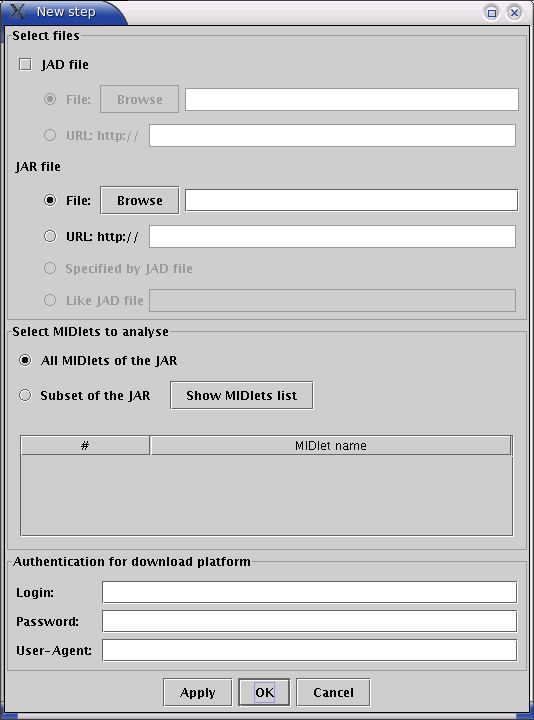
\includegraphics{figures/GUI-new-step-dialog}}
\end{center}
\caption{Specify the new step properties}
\label{figNewStep}
\end{figure} 

The properties dialog depicted on figure
\ref{figNewStep} is
raised so you can specify parameters of the new analysis. When you
click \texttt{Apply} or  \texttt{OK}, a new step will be added to the
current check-list. 

The first section of the dialog allows you to
specify the JAD and the JAR files to analyse. The JAD file is
optional, whereas the JAR is mandatory. The goal here is to inform the
\ma where to find the wanted files. To do so, you may either specify a
local path (\texttt{File}) or an HTTP address (\texttt{URL}) to the
file. If you specify a JAD file, then the location of the JAR can be
specified relative to the JAD location: you can indicate that the JAR
is to be found at the same location as the JAD's (select \texttt{Like
  JAD file} option), or at the location \emph{that is specified in the
  JAD file}, namely at the address assigned to the
\texttt{MIDlet-Jar-URL} attribute of the JAD (select \texttt{Specified by
JAD file}).

The second section lets you specify which MIDlets of the JAR file
should be analysed. Indeed, a JAR may define more than one
MIDlet object, although it often contains only one. By default, all
MIDlets of the selected JAR will be analysed (even hidden ones). To choose a
subset, select \texttt{Subset of the JAR} and press \texttt{Show MIDlets
 list}. The tool will look for the JAR file, look into it and tell you the list
 of \emph{visible} MIDlets that it contains.  
 From that point, only the MIDlets that you select from that list will be taken into account.

Some downloading platforms require an authentification to access it. The third
section allows you to specify a login, a password and a user-agent to use when
downloading JAD and JAR files. 


\subsubsection{Adding an APK}
The dialog (figure \ref{figStepAndroid}) is much simpler as there is only one
file. It is either a local file or a URL. If it is a URL, it is possible to give some credentials to perform the
download. 

\begin{figure}[ht]
\begin{center}
\scalebox{0.5}{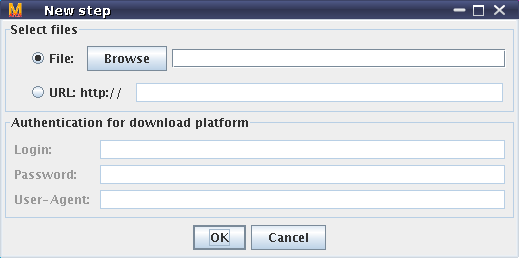
\includegraphics{figures/GUI-new-step-android}}
\end{center}
\caption{Specify the new step properties for an APK}
\label{figStepAndroid}
\end{figure} 
\subsection{The \texttt{Edit} Menu} \label{EditMenu}
\begin{itemize}
\item{\textbf{Select all}} Select all steps of the check-list.
\item{\textbf{Unselect all}} Unselect all steps of the check-list.
\item{\textbf{Copy}} Register in memory the selected steps.
\item{\textbf{Paste under}} Paste all steps previously registered with the
\texttt{Copy} option under the last selected row. 
\item{\textbf{Remove}} Remove the selected steps from the check-list.
\ifthenelse{\equal{\Gallery}{true}}{
\item{\textbf{Remove associated steps}} Remove all steps from the check-list
table which are associated with selected editor's list(s) in the editor's list
table. }{}
\item{\textbf{Properties...}} Edit the properties of the selected
step. The dialog that opens is very similar to the one used at step-creation
time (see section \ref{FileMenu}, figure \ref{figNewStep}). When you
press \texttt{Apply} or \texttt{OK}, your changes are applied to the
selected step.
\item{\textbf{Configuration...}} Edit the global configuration options of the
\ma. This window contains four tabs.
\begin{itemize}
  \item The ``Main'' tab (see figure \ref{MainTabOfConfigDialog})
	\begin{itemize}
  	 	\item \textbf{Default profile}: The default profile selected in the combo
  	box of the check-list zone at the opening of the \ma.
  		\item \textbf{Download of files} Select a proxy if it is necessary.
  		\item \textbf{Custom} The Cascading Style-Sheet (CSS) file to use for
  		pretty-presentation of the HTML reports. The default one is provided to you
  		with the \ma.
    \end{itemize}
    \begin{figure}[ht]
		\begin{center}
		\scalebox{0.5}{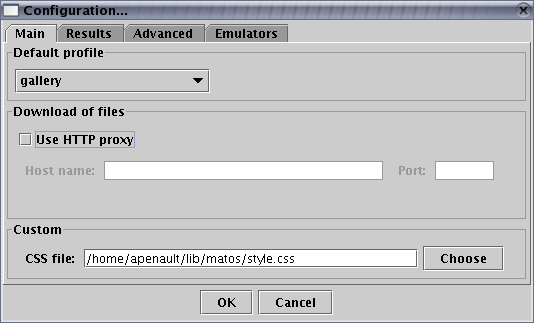
\includegraphics{figures/MainTab}}
		\end{center}
		\caption{The ``Main'' tab of the configuration's window}
		\label{MainTabOfConfigDialog}
	\end{figure}
  \item The ``Results'' tab (see figure \ref{ResultsTabOfConfigDialog})
      \ifthenelse{\equal{\Gallery}{true}}{
      	%\item \textbf{Storage}: 
      	
      
      	The first option ``Use archiving database to store analysis results''
      	allows to register all analysis results in the database. If this option
      	is selected and a connection to a database is available, you can ask to
      	the \ma to retrieve previous results from database. In that case, when a
      	step is added in the check-list, the \ma looks for previous results for
      	this JAR file in the database. If it finds a result, it displays its
      	verdict. If parameters of current step is a little different to the
      	registered result, it puts a ``M'' in the fourth column of the check-list
      	and indicates differences in associated tool tip in red. Moreover, you
      	can configure database parameters i.e. its URL (like 
      	\emph{jdbc:mysql://localhost/matos}), a user login and a user password to
      	access to the database by clicking on ``Configure database" button.
      	
      	The second option (``Use a directory to store analysis results''),
      	selected by default, allows you to select a directory to store analysis
      	results. If this option is selected, all generated reports are registered
      	in the specified directory. For more information on working of this
      	directory, please refer to \ref{HTMLReportGeneration}. 
      	
      	If you choose the ``Don't store analysis results'' option, results are
        registered in a temporary directory during the execution of the \ma,
        this directory will be deleted at the closing of the \ma.  
        
        If the first option is selected and the database connection is not
        available, the behaviour of the \ma is the same that if the third option
        is selected i.e. analysis results are stored in a temporary directory
        that is deleted at the closing of the \ma.
%         \item \textbf{Retrieving}: If a connection to a database is available, you
%         can ask to the \ma to retrieve previous results from database. If the
%         option is selected, when a step is added in the check-list, the \ma
%         looks for previous results for this JAR file in the database. If it
%         finds a
%         result, it displays its verdict. If parameters of current step is a 
%         little different to the registered result, it puts a ``M'' in the fourth
%         column of the check-list and indicates differences in associated tool
%         tip in red.
%         \item \textbf{Configure database\ldots}: This button allows you
%         configuring database parameters i.e. its URL (like
%         \emph{jdbc:mysql://localhost/matos}), a user login and a user password
%         to access to the database.
        \begin{figure}[ht]
			\begin{center}
			\scalebox{0.5}{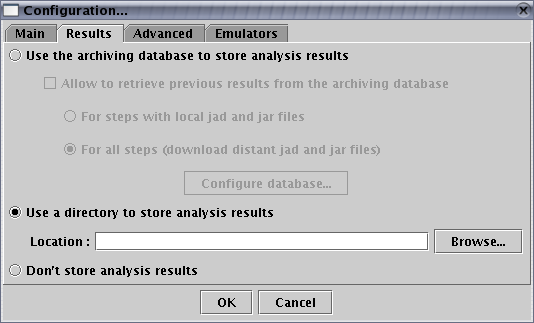
\includegraphics{figures/ResultsTabGallery}}
			\end{center}
			\caption{The ``Results'' tab of the configuration's window}
			\label{ResultsTabOfConfigDialog}
	   	\end{figure}
      }{
       By default, HTML reports are stored in the directory specified during the
       installation and all generated reports are registered in it. If you 
       choose the ``Don't store analysis results'' option, results are 
       registered in a temporary directory during the execution of the \ma, this
       directory will be deleted at the closing of the \ma. Please refer to
       \ref{HTMLReportGeneration} for information on HTML reports. \begin{figure}[ht]
			\begin{center}
			\scalebox{0.5}{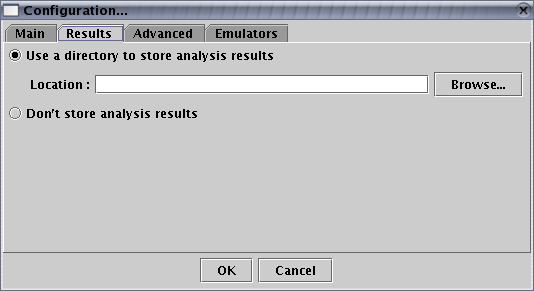
\includegraphics{figures/ResultsTab}}
			\end{center}
			\caption{The ``Results'' tab of the configuration's window}
			\label{ResultsTabOfConfigDialog}
	   	\end{figure}
	  }
  \item The ``Advanced'' tab (see figure \ref{AdvancedTabOfConfigDialog})
  	\begin{itemize}
       \item \textbf{Add directories}: If the \texttt{Yes} option is selected
       in the ``Advanced'' tab, the \ma will consider during loading a directory
       that a JAR and a JAD file which have the same name (like Pacman.jad and
       Pacman.jar) are relative to the same MIDlet suite. By default, the
       \texttt{No} option is selected.
       \begin{figure}[ht]
			\begin{center}
			\scalebox{0.5}{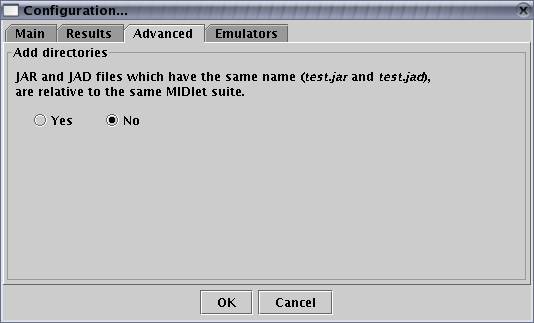
\includegraphics{figures/AdvancedTab}}
			\end{center}
			\caption{The ``Advanced'' tab of the configuration's window}
			\label{AdvancedTabOfConfigDialog}
	   	\end{figure}
      \end{itemize}
  \item Finally, the ``Emulators''tab (see figure \ref{EmulatorTabOfConfigDialog})
		
		In this tab, you can manage emulators that allow to run MIDlets of the
		check-list. The ``Add emulator'' button displays a dialog to make a link to a
		new emulator by giving a name and its command line to run it. The
		command line must contains ``\%JAD\%'' string to indicate where the path to
		the JAD must be given in it.
		The ``Remove emulator'' button allows to remove the emulator selected in the
		combo box.		
		The ``Edit emulator's properties'' button allows to modify properties of
		selected emulator i.e. its name and/or its command line.		
		The emulator selected in the combo box is the emulator run by default when you
		launch the emulator by a right click on a MIDlet suite.
		
		\begin{figure}[ht]
			\begin{center}
			\scalebox{0.5}{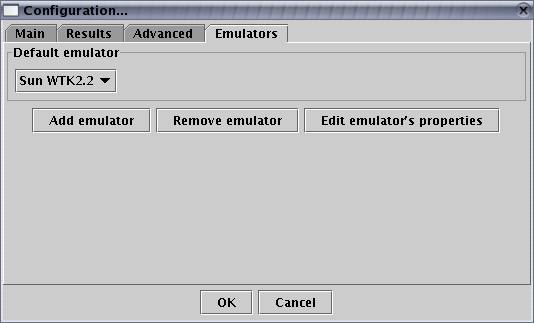
\includegraphics{figures/EmulatorTab}}
			\end{center}
			\caption{The ``Emulators'' tab of the configuration's window}
			\label{EmulatorTabOfConfigDialog}
	   	\end{figure}
\end{itemize}
\end{itemize}

\ifthenelse{\equal{\Gallery}{true}}{
\subsection{The \texttt{View} Menu}
The editor's list gives more information about MIDlet suite than information
given by columns of the check-list table. You can see all retrieved information
from Excel files by selecting \texttt{Complete information} in the \texttt{View}
menu. By default, the showed view is \texttt{Basic information} which contains
uniquely previously described columns. The columns added by selecting
\texttt{Complete information} are:

\begin{itemize}
\item{\textbf{EL\#}} Number of associated editor's list.
\item{\textbf{Name}} Name given by the editor to the MIDlet suite.
\item{\textbf{SMS}} True if the MIDlet suite makes SMS connection(s).
\item{\textbf{Authorized URLs}} By default, HTTP connections are forbidden. To
authorize HTTP connections to some URLs, the editor can declare these URLs in
the editor's list.
\item{\textbf{Service}} Name of editor's service.
\item{\textbf{Version}} Version of the given MIDlet suite.
\item{\textbf{Terminal}} Compatible devices with this MIDlet suite.
\end{itemize}
}{}

\subsection{The \texttt{Tools} Menu}
\begin{itemize}
\item{\textbf{View latest report}}: Displays the latest generated report for
the selected step.
\item{\textbf{View JAD}}: Displays the contents of the JAD file associated
to the selected step.
\item{\textbf{View JAR manifest}}: Displays the contents of the JAR manifest 
file associated to the selected step.
\item{\textbf{Analyse selection}}: Starts the analysis process for
the selected step(s) only. 
\item{\textbf{Analyse all}}: Starts the execution of the entire
check-list. All steps are processed.
\item{\textbf{Confirm the verdict}}: You can confirm the verdict given by the
\ma. In that case, the verdict's cell appears with a green background.
\item{\textbf{Modify the verdict}}: You can also modify the verdict given by the
\ma. The verdict in the ``Verdict'' column will be the verdict given by you and
the cell's background will be in red.
\item{\textbf{View statistics}}: Displays a graphic which represents verdicts in
the current check-list.
\item{\textbf{View log file}}: You can show trace generated by the \ma showing
this file.
\ifthenelse{\equal{\Gallery}{true}}{
\item{\textbf{Management tools}}: This menu allows to access to the database
management tool. It enables you showing and removing information registered in
database. To have more details, see section \ref{databaseManagementTool}.
}{}    
\item{\textbf{Launch selected MIDlet suite}}: Displays a submenu which contains
the name of available emulators. You could add a new emulator by clicking on
``Add emulator\ldots'' button and giving a name and its command line to run it.
\end{itemize}

\subsection{The \texttt{Packages} Menu}
This menu allows to select what set of Java distributions (JSRs) must be taken
into account during analysis. In general, keep \texttt{all} selected.

\subsection{The \texttt{Help} Menu}
\begin{itemize}
%\item{\textbf{User's manual}}: Opens the online help.
\item{\textbf{About}}: General information about the \ma tool.
\end{itemize}

\ifthenelse{\equal{\Gallery}{true}}{

\subsection{ The Database Management Tool} \label{databaseManagementTool}

The Database Management Tool is composed in three parts and a menu bar. It
allows to view results stored in database by selecting criteria and gives the
possibility to remove results from the database.

\subsubsection{Selection criteria}

The ``Criteria'' panel (see figure \ref{criteriaPanel}) allows to give selection
criteria to retrieve steps from database and to display them in the ``Results''
panel.

The selection criteria are:
\begin{itemize}
  \item{\textbf{Profile}} the analysis profile.
  \item{\textbf{Version}} the version of selected profile.
  \item{\textbf{Verdict}} the verdict given by the \ma.
  \item{\textbf{User verdict}} the user verdict i.e. if the verdict given by the
  \ma is confirmed, modified by you or you don't put your own verdict for these
  steps.
  \item{\textbf{Midlet Analyser release}} release of the \ma.
  \item{\textbf{JAR name}} you have three possibilities to give name of JAR file
  you want to retrieve from database. Either you give a part of JAR name or
  the beginning or the end of JAR name.
  \item{\textbf{Date}} you can also retrieve steps by creation date of results.
\end{itemize}

\begin{figure}[ht]
	\begin{center}
	\scalebox{0.5}{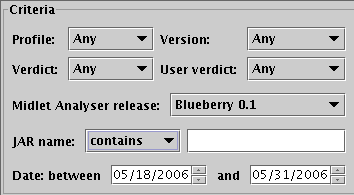
\includegraphics{figures/CriteriaPanel}}
	\end{center}
	\caption{``Criteria'' panel of the Database Management Tool}
	\label{criteriaPanel}
\end{figure}

\subsubsection{Steps' presentation}

Steps retrieved from database are displayed in the ``Results'' panel. To update
the list of steps after a modification of criteria, click on the ``Refresh''
green button above this panel. The table in this panel is similar to the table
in the check-list zone but another column indicates the creation date of
analysis reports (see figure \ref{resultsPanel}).

\begin{figure}[ht]
	\begin{center}
	\scalebox{0.5}{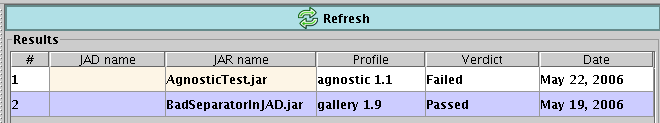
\includegraphics{figures/resultsPanel}}
	\end{center}
	\caption{``Results'' panel of the Database Management Tool}
	\label{resultsPanel}
\end{figure}

\subsubsection{Step's properties}

A third panel allows to display properties by selecting a step in ``Results''
panel (see figure \ref{stepProperties}).

\begin{figure}[ht]
	\begin{center}
	\scalebox{0.5}{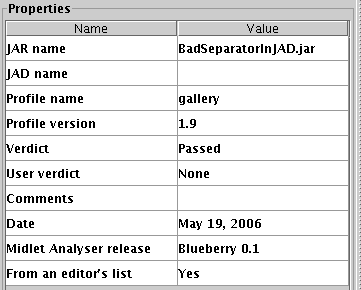
\includegraphics{figures/stepPropertiesPanel}}
	\end{center}
	\caption{``Properties'' panel of the Database Management Tool}
	\label{stepProperties}
\end{figure}

\subsubsection{Menus}

\begin{itemize}
  \item{\textbf{File -> Quit}} Close the Database Management Tool.
  \item{\textbf{Edit}}
	\begin{itemize}
      \item{\textbf{Select all}} Select all steps of the results' table.
      \item{\textbf{Unselect all}} Unselect all steps of the results' table.
      \item{\textbf{Remove selection}} Remove selected step(s) from database.
      \item{\textbf{Remove by date\ldots}} Display a window which enables to
      remove either all steps whose creation date is between two dates or before
      a specified date or older than \emph{n} days.
      \item{\textbf{Database properties\ldots}} Display a window which enables to
      configure the database URL, the database user login and the database user password.
    \end{itemize}
  \item{\textbf{Tools -> View report}} Enable to view the analysis report of the
  selected step.
\end{itemize}

}{}

\section{Analysis Profiles}\label{AnaProfs}

Most of the analysis done by the \ma is performed according to an
analysis profile. An analysis profile is a text file where directives
for the tool are specified, where you can define what the analysis must
focus on, and also how the results of the analysis should be
presented. Multiple profiles can be defined for different purposes,
but the \ma is always bound to a single profile at a time. 

An analysis profile can be seen as the implementation of a
set of analysis rules. The profile describes, in short terms, what
Java methods and arguments must be studied (it declares sort of
``probes'' on these objects), and according to the results observed,
what text messages must be produced in the report. However, in
contrast to a probe which usually provides a sample of the possible
objects states (a thermometer, for instance, indicates the current
temperature, but not tomorrow's temperature), the \ma's probes give
you a pattern covering all possible states, taking into
account all possible executions of the application. The pattern tries
to stick as much as possible to the real set of possible values, but
in general this exact set of values can not be computed; that's why
the analysis returns an upper approximation of the set, to make sure
at least that all possible values are captured.

Modifying a profile should be done very carefully, since it widely
determines the analysis engine's behaviour. If you deal with the
analysis of particularly critical features, make sure your
specification of the associated rules is correct and won't lead to
confusion between what you had in mind and what the tool
understands. On the other hand, this open approach is very flexible
and allows to highly customize the targets, preciseness and
presentation of your reports. We recommend that you contact us for
assistance if you wish to do changes to your profile, or define your
own profile from scratch. Section \ref{ProfFormalization} presents how
to formalize a profile.


\subsection{The MIDP Agnostic profile}

The \ma comes with a predefined profile called Agnostic. Its purpose
is to report the use of a set of potentially critical features, mainly
related to inputs/outputs (I/O) : network connections, system properties queries, Record Management
System (RMS), multimedia players, etc. The main characteristic of the Agnostic
profile is that results are not judged: there's no notion of pass or
fail, but just reporting.

The observed methods are the following, with the observed argument(s)
shown in bold-face when there are more than one:

\begin{itemize}
\item \texttt{javax.microedition.io.Connector.open(java.lang.String)}
\item \texttt{javax.microedition.io.Connector.open(\textbf{java.lang.String},int)}
\item \texttt{javax.microedition.io.Connector.open(\textbf{java.lang.String,int},boolean)}
\item \texttt{javax.microedition.io.Connector.openDataInputStream(java.lang.String)}
\item \texttt{javax.microedition.io.Connector.openDataOutputStream(java.lang.String)}
\item \texttt{javax.microedition.io.Connector.openInputStream(java.lang.String)}
\item \texttt{javax.microedition.io.Connector.openOutputStream(java.lang.String)}
\item \texttt{javax.wireless.messaging.MessageConnection.newMessage\\ \mbox{} \hspace{1cm} (java.lang.String,\textbf{java.lang.String})}
\item \texttt{javax.wireless.messaging.Message.setAddress(java.lang.String)}
\item \texttt{com.siemens.mp.gsm.SMS.send(\textbf{java.lang.String},java.lang.String)}
\item \texttt{com.siemens.mp.gsm.SMS.send(\textbf{java.lang.String},byte[])}
\item \texttt{com.siemens.mp.io.Connection(java.lang.String)}
\item \texttt{javax.microedition.media.Manager.createPlayer(java.lang.String)}
\item \texttt{javax.microedition.media.Manager.createPlayer\\ \mbox{} \hspace{1cm} (javax.microedition.media.protocol.DataSource)}
\item \texttt{javax.microedition.media.protocol.DataSource(java.lang.String)}
\item \texttt{javax.microedition.rms.RecordStore.openRecordStore\\ \mbox{} \hspace{1cm} (java.lang.String,boolean,\textbf{int},boolean)}
\item \texttt{javax.microedition.rms.RecordStore.setMode(\textbf{int},boolean)}
\item \texttt{java.lang.System.getProperty(java.lang.String)}
\item \texttt{java.lang.Class.forName(java.lang.String)}
\item \texttt{javax.microedition.midlet.MIDlet.platformRequest(java.lang.String)}
\end{itemize}


\section{Analysis Reports}

When you select a step in the check-list then ask \texttt{View latest
report}, a tab in your default browser will open to display the latest results
of that analysis. Note that the presentation style can be customized by changing the CSS file
(cf. \ref{EditMenu}). In this section we explain the structure of a
report, and how reports are stored on your disk, so you can open them
outside of the \ma application.

\subsection{Structure of a Report}

A MIDP report mainly contains three sections.

\begin{itemize}
\item\textbf{Header}: General information on the analysis.
\item\textbf{Descriptors conformity}: Remarks on JAD file and JAR manifest
  validity, and if both are given, on their consistency. 
\item\textbf{Per-MIDlet results}: For each MIDlet analysed, this section
  presents all remarks coming out of the Features Usage analysis
  phase. Messages displayed at that level are
  defined in the analysis profile used. 
\end{itemize}

An Android report mainly contains two sections.
\begin{itemize}
  \item \textbf{Header}: General information extracted from the manifest
  \item \textbf{A global analysis} of the APK. 
\end{itemize}
It is possible to get a per component analysis of an APK but it is not clear
that this distinction is worth the effort (the analysis time is almost
multiplied by the number of components).

% \subsection{The \texttt{Report} window} \label{ReportWindowSection}
% 
% This window gives access to a \texttt{File menu} which contains three options: 
% \begin{itemize}
%   \item \textbf{Export report in HTML\ldots} Display a dialog which allows to select
%   an HTML file to save the report.
%   \item \textbf{Export report in PDF\ldots} Display a dialog which allows to select
%   a PDF file to save the report.
%   \item \textbf{Close} Close this window. You can also close it by
%   clicking on the \texttt{Close} button at the bottom of this window.
%   \begin{figure}[ht]
% 	\begin{center}
% 	\scalebox{0.5}{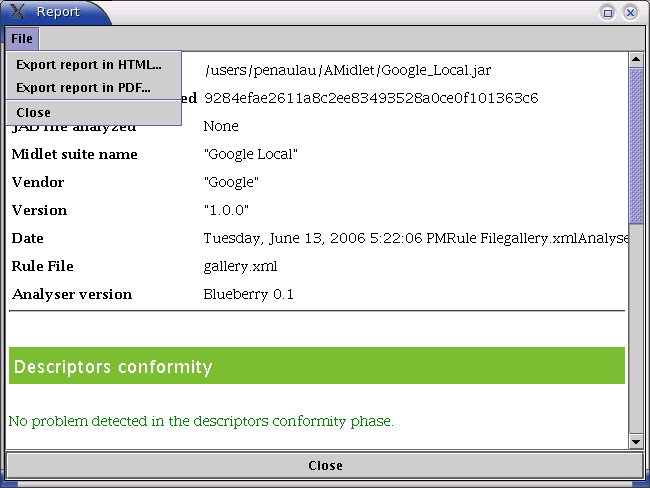
\includegraphics{figures/ReportWindow}}
% 	\end{center}
% 	\caption{The ``Report'' window}
% 	\label{ReportWindow}
%   \end{figure}
% \end{itemize}

\subsection{Using Reports Outside of the Tool} \label{HTMLReportGeneration}

If you chose to store analysis results in a directory in the configuration's
window (see section \ref{EditMenu}), the \ma will create
a sub-folder called \texttt{AnalysesResults} into the specified directory at the
first analysis. In the \texttt{AnalysesResults} folder the tool then generates a
new subfolder \texttt{Results\emph{<i>}} for each new execution of the analysis
process, ie. for each new execution of a check-list.
 
For each execution, there are: 
\begin{itemize}
\item one HTML report per step executed, and
\item one summary file (\texttt{index.html}) pointing to all the HTML reports
\end{itemize}

% As the execution of the
% check-list goes along, the \ma creates a sub-folder called
% \texttt{AnalysesResults} into \textbf{output directory} specified in the
% configuration of the tool. Refer to section \ref{EditMenu} to learn how to
% customize the output directory. 
% In the \texttt{AnalysesResults} folder the tool then generates a new
% subfolder \texttt{Results\emph{<i>}} for each new execution of the
% analysis process, ie. for each new execution of a check-list. The
% \emph{i} counter contains all result files for the execution number \emph{i}, namely:
% \begin{itemize}
% \item one HTML report per step executed, and
% \item one summary file (\texttt{index.html}) pointing to all the HTML reports
% \end{itemize}

If you open \texttt{index.html} in your HTML
browser, you'll find something very similar to the check-list zone
available in the GUI. You can then print reports from there. It is the
responsibility of the user to clean the execution folders
that are no longer needed.

% If you chose the ``Don't store analysis results'' option in the configuration's
% window, you can still save results explicitely choosing \texttt{File -> Export
% report in HTML\ldots} or \texttt{File -> Export report in PDF\ldots} menu in
% the \texttt{Report} window (see section \ref{ReportWindowSection}).

 %%% Local Variables: 
%%% mode: latex
%%% TeX-master: "Users-manual"
%%% End: 

%===========================================================================
\chapter{Customization of security profiles} \label{AdvancedUsage}

In this section, we present more technical things, that you normally
won't have to use every day. We explain how to understand analysis
profiles and to write your own profile and present further
configuration options.

\section{Analysis Profiles Specification}\label{ProfFormalization}
In this section, we present what can be specified in a profile and the
syntax to do so.

\subsection*{WARNING} 
\begin{itemize}
\item France Telecom publishes the specification of
  analysis profiles for your convenience. However, be advised that this
  specification may change in the future. 
\item If you change your analysis profiles, please keep in mind that
  profiles widely condition the behaviour of the tool's
  engine. Therefore, any change should be carefully understood and
  validated prior to any operational usage. \textbf{France Telecom rejects any
  responsibility in case of problems resulting from the bad
  interpretation of the specification's semantics}. Cf. also
  \ref{AnaProfs}. However, we can provide assistance in this task and
  do the changes for you.
\end{itemize}

\subsection{How Are Profiles Stored?}
Analysis profiles are XML files that must be placed in
\texttt{lib/definitions} folder of your installation directory on
Windows (\texttt{lib/matos/definitions} folder on Linux).

\subsection{What's In a Profile?}
A profile basically lets you define 4 things:
\begin{itemize}
\item \textbf{Header}: General information on the profile.
\item \textbf{Options}: To overload options set by default in the tool's
configuration.
\item \textbf{Rules}: To define the Java methods to be watched
during the Features Usage phase.
\item \textbf{Reports}: To associate messages to some result values (what messages
should be raised according to the results obtained).
\end{itemize}

\subsection{Syntax by the Example}\label{ProfSyntax}

\subsubsection{Header}
A profile typically starts as shown below. The two first lines are
mandatory and must be written as shown. In the \texttt{<matos>}
tag, you're required to specify at least a name for the profile.
The \texttt{</matos>} closing tag must appear at the very end of
the file. Your entire profile data will be specified inside the
\texttt{<matos>} element.

\begin{verbatim}
  <?xml version='1.0' encoding='utf-8'?>
  <!DOCTYPE matos SYSTEM "../matos.dtd">

  <matos name="MyProfile"
         description="The purpose of the present profile is..."
         version="1.5"
         date="18.08.2006">
\end{verbatim}

\subsubsection{Options} \label{optionsSecurityProfile}
Configuration options may be set for a profile. The options you can
set are those presented in \ref{AdvConfigOptions}. Values set in a
profile take precedence over those set as defaults in the configuration
file.
\begin{verbatim}
  <option name="anasoot.treatConcatenation" value="false">
      <description>
        This option controls if a special treatment is applied to the
        <code>StringBuffer.append</code> method. In this profile, string 
        concatenation is not treated.
      </description>
  </option>
\end{verbatim}

\subsubsection{Syntax of method signatures}
We often need to specify methods. For this, we use the signature  of the method.
The signature is the description of the name and types of arguments and
result. The syntax is the following:
\begin{verbatim}
resultType methodName(argType1,...,argTypen)
\end{verbatim}
Note that the number of spaces is significant and that you can only put one
space after the result type. Types are fully qualified names for classes and
are the class name followed by the correct number of [] for array types. 
The name of primitive type is the regular java name.

\subsubsection{Rules (probes)}
A rule defines a particular observation target for the Features Usage
phase, namely a method identifier plus the arguments of that method to
be observed. Conceptually, a rule can be seen as a probe on the
defined target.

In the following example, we define a rule that will check how the
MIDlet uses the network connection feature, with a focus on the
address used in the connection. This address is passed through the
argument number 1 of the method. Values returned by this rule will be
reported using the report called \texttt{net}. The description element
is always optional.
\begin{verbatim}
 rule name="connection">
  <description>
    This rule is to observe what addresses are used when the
    midlet tries to open a network connection.
  </description>
  <args class="javax.microedition.io.Connector"
    signature="javax.microedition.io.Connection open(java.lang.String)"
    report="net">
     <argument position="1"/>
  </args>
</rule>
\end{verbatim}

In fact there are three types of rules:
\begin{itemize}
\item{\textbf{Observation of method argument(s)}}: this is the above
  example. Note that the fully-qualified identifier of the target
  method must be given (absolute package path expected for all types).
  Multiple \texttt{argument} elements can be specified if
  multiple arguments are to be observed. Arguments are numbered
  starting from 1, from left to right. 
% TODO: COMPRENDRE PUIS TRADUIRE: La position 0 correspond � l'objet
% racine de l'appel (\texttt{this}).
\item{\textbf{Observation of a class field}}: in the following
  example, we define a probe on the field \texttt{name} of the class
  \texttt{Person}. Here again, types must be fully-qualified.
\begin{verbatim}
  <rule name="peoplesName">
    <field class="myPackage.Person" type="String name"/>   
  </rule>
\end{verbatim}
\item{\textbf{Observation of a method's return value}}: in the
  following example, we define a probe that provides the values
  returned by the method that gives the name of a record
  store.
\begin{verbatim}
  <rule name="recordStoreName">
    <return class="javax.microedition.rms.RecordStore" 
            type="java.lang.String getName()"/>   
  </rule>
\end{verbatim}
\end{itemize}

\subsubsection{Reports}
As seen above, each rule is associated to a report element. The report
defines what messages will be produced according to those
results. 
Reports are identified by names. There can be only one report with a
given name and it is the first defined that takes precedence.
Besides the name attribute, there is an optional alias attributes that
can defines a comma separated list of alternate names. This is useful
to override a list of automatically generated reports with 
one defined by hand.

There are three types of report:

\begin{itemize}
\item{\textbf{Pseudo constant report}}: a report that offers a choice
  among 2 bodies (messages). If ALL possible values of the observed data -- the
  probe's target -- turned out to be fully determined, the
  \texttt{pass} body is displayed. If at least in one case, the value
  failed to be fully computed, then the \texttt{fail} message is
  produced.
\begin{verbatim}
  <report name="R1">
    <pseudoConstant>
      <fail> 
        In some cases, the argument(s) passed to method %C.%M
        can't be fully determined.
      </fail>
      <pass> 
        Managed to compute <b>all</b> possible values of observed 
        argument(s). 
      </pass>
    </pseudoConstant>
  </report>
\end{verbatim}
Each message is actually a piece of HTML code (notice the \texttt{<b>}
bold-face tag in the example above). Besides,  note that we use some
additional non-HTML tags: \texttt{\%C} and \texttt{\%M}. They are
interpreted by the report generator, and are explained further;
however, these special tags can't be used in the \texttt{pass} message
part.

\item{\textbf{Pseudo string report}}: a report that offers a choice
  among N messages. Each message is associated to a filter, and for
  each value computed, filters are evaluated one by one (following the
  order in which they are declared), until the value matches one of
  them, in which case the associated message is displayed. Filters are
  regular expressions (patterns).
\begin{verbatim}
  <report name="netS">
    <description>
      This report extracts information on the schemes used in the URL.
    </description>
    <pseudoString>
      <filter pattern="\x22([^:]*):([^\x22]*)\x22">
        <b>The application opens a network connection:</b>
        <ul> 
          <li> Method called: %C.%M </li>
          <li> Method hosting the call: %c.%m </li>
          <li> URL used: <b>%r</b> </li>
          <li> Connection type: <b>%1</b> </li>
        </ul>
      </filter>
      <filter pattern=".*">
        <b>The application opens a network connection (but of
           an <font color="red">unknown type</font>):</b>
        <ul> 
          <li> Method called: %C.%M </li>
          <li> Method hosting the call: %c.%m </li>
          <li> URL used: <b>%r</b> </li>
        </ul>
      </filter>
    </pseudoString>
  </report>
\end{verbatim}
Note that the second filter here is associated to the \texttt{''.*''}
expression that means ``anything else''. A special filter called \texttt{default}
also means ``anything else'', but is produced only once even if many
values can't be matched by any filter above, while the \texttt{''.*''}
case is produced for every such value. 
\begin{verbatim}
    ../..
    <pseudoString>
      <filter pattern="\x22([^:]*):([^\x22]*)\x22">
         (The message body)
      </filter>
      <filter ../..>

      <default> Oops... no expression matched in report R1! </default>
    </pseudoString>
\end{verbatim}
Filters are now named. When one use the XML output, the result will only
contain the name of the filter that matched.
\item{\textbf{Simple message}}: a report that just print a message. But this
message may refer to the argument. For example to print all the potential values
of this argument without filtering. The only useful macros are therefore 
  \begin{itemize}
    \item \texttt{\%r} the complete value
    \item \texttt{\%C}, \texttt{\%M} and \texttt{\%S} the specification of the
    method called.
    \item the specification of the caller method.
  \end{itemize}
\begin{verbatim}
     <message>The list of objects used : %r </message>
\end{verbatim}
  You can put simple HTML in the message definition. If HTML is not
  well-balanced XML, you must escape the HTML entities (replace $<$ with
  \verb!&lt;!)
\item{\textbf{Forbidden method message}}: a report that prints a message when a
forbidden method is used. 
  \begin{itemize}
    \item \texttt{\%p} the list of program points where it is used.
  \end{itemize}
\begin{verbatim}
     <message>The method is called at the following points: %p
     </message>
\end{verbatim}
  
\item{\textbf{Conjunction report}}: a report that compiles the output
  of two other reports. The first report is executed, then the second
  one. However, if the first one is a pseudo constant
  report that fails, the second report is not produced. The reason for
  this behaviour is that it makes no sense to perform pattern matching
  on a value if we failed to fully establish that value.

\begin{verbatim}
  <report name="net">
    <conjunction>
      <ref name = "R1"/>
      <ref name = "R2"/>
    </conjunction>
  </report>
\end{verbatim}
    
  Rules may give back results on several arguments but report should only refer
  to one argument at a time. This is the only report where you can specify the
  position of the argument that must be checked (as a number between 0 and the
  number of arguments checked by the rule).
  
  If conjunction reports are included into other conjunction report, the
  position should usually only be specified in the first. The element is then
  immediately filtered.
  
  For example if you have a rule that check two arguments you can build two
  filters \texttt{F0} and \texttt{F1} for each argument and a simple message
  report \texttt{M} to print information on the function. The final report
  \texttt{R} will be built as:
\begin{verbatim}
  <report name="R">
    <conjunction>
      <ref name = "M"/>
      <ref name = "F0" pos="0"/>
      <ref name = "F1" pos="1"/>
    </conjunction>
  </report>
\end{verbatim}
  Please note that the positions given here refer to the positions in the result
  row.  It is not the position of the argument in the call of the method
  analyzed.
\end{itemize}

\subsubsection{Structure element}
This is a feature introduced with Android profile. The structure element
describes how the report is organized. It contains an HTML body where some tags
specify where to put the result of a given analysis. The tags are
\verb!<callRef name="..."/>! and \verb!<fieldRef name="..."/>! where the
attributes is the name of the rule (not the report) to inline at this point.
It can also contain \verb!<sdiv>! elements. An SDIV is a division that is
displayed only if there is a content in it: at least one of the rules that is
specified with callRef or fieldRef has a result to display. An sdiv element
may be named (optional \verb!name! attribute). Finally the \verb!<nodes/>!
element is used to declare the location where the node table must be inlined.

Note that the Android profile also contains some JavaScript to make it possible
to have foldable explanations. The JavaScript is tailored to handle two
languages. Contents must be defined in contiguous sections (using a \verb!div!
element) whose class are respectively \verb!AuxFoldBox! and \verb!FoldBox!).

\subsubsection{The score section}
The \verb!score! tag introduces a basic scoring mechanism for Anasoot. The score
section contains score elements that describes the individual contributions and
text that is only used in the documentation of the profile. The score element
has one attribute \verb!threshold! defining the value above which the analysis
is considered as failed.

Each score element has a name (attribute \verb!name!), a message (attribute
\verb!message!) and a score value (attribute \verb:score:). The name is used to
refer to the score element in other elements. The message is the text displayed
in the report. The score is the contribution of the element to the global score.
If it is 0 (no contribution), the element is NOT displayed. But it is still
marked as triggered and may be used by other elements (any-of and all-of).

The tags used to describe score elements are the following :
\begin{itemize}
  \item \verb!stringmatch! matches a string in the report. The element uses a
  \verb!pattern! attribute describing a regular expression (in Java regexp
  format with special characters escaped in XML format). Do not use patterns
  spanning over multiple results as in fact the search is local to an element.
  \item \verb!rulematch! element contains a list of \verb!rule! element
  characterized by a \verb!name! attribute. This element is triggred if any of
  the rules has been triggered during the analysis. A rule name is either an
  Anasoot rule or the name of an \verb!sdiv! section grouping several rules. The
  section is considered as trigered if any of the rules it contains has been
  trigered.
  \item \verb!any-of! is trigered if any of the score elements it refers to has
  been trigered. Score element are identified by the \verb!element! tags. These
  tags contain a \verb!name! attribute.
  \item \verb!all-of! is trigered if all of the score elements it refers to have
  been trigered. It is similar to \verb!any-of!
  \item \verb!permission! matches a permission in the manifest. The full name of
  the permission must be given in the \verb:perm: attribute.
  \item \verb!catcher! are special elements. They have no score and no name.
  They are used to print the list of elements in the report matching the
  \verb!pattern! attribute. The \verb!message! attribute is the text printed as
  header for this section.
\end{itemize}


\subsubsection{Score element}


\subsubsection{Global structure of HTML report}
The report should be a compliant XHTML document. So that automatic XSL
transforms can be done on the document, we have introduced a few division in the
generated report whose class attribute can be used to select the division
content.

The following class are used in the report:
\begin{itemize}
  \item header : the header part of the report (MIDP or Android)
  \item compatibility : indication on hidden APIs used in an Android report
  \item score : the score and how the score is split between subelements
  \item catched : the substring that are isolated at the end (for example URLs)
  \item AndroidManifest : the manifest analysis
  \item android : main analysis.
\end{itemize}

\subsection{Customization of descriptors conformity phase}
\label{CustoConform}

To add properties to respect for the descriptors conformity phase, options
described in section \ref{optionsSecurityProfile} are used. You can add
some properties of JAD file and/or JAR manifest file about:
\begin{itemize}
  \item Line end characters.
  \item Order of attributes.
  \item Mandatory attributes.
  \item Forbidden attributes. 
\end{itemize}

\subsubsection{Line end separator}
According to the operating system, the line end character could be only
\texttt{CR LF} (\verb!\r\n!), \texttt{CR} 
(\verb!\r!) or \verb!LF (\n)!. The MIDP 2.0 specification
authorizes only to use \texttt{CR LF} or \texttt{LF} character as end of line in
the JAD file. You can specify only a subset of these characters as
authorized line end separator for the descriptors. The given characters must be
separated by a comma.\\
Because the security profile is written in XML, the line end characters must be
coded like indicated below:
\begin{itemize}
  \item{CR LF}: \verb!&#x000D;&#x000A;!
  \item{CR}: \verb!&#x000D;!
  \item{LF}: \verb!&#x000A;!
\end{itemize}

For instance,
\begin{verbatim}
  <option name="descriptor.jad.endline" value="&#x000D;&#x000A;">
    <!-- This option defines that the only authorized character to 
         mark the end of line is CR LF -->
    <description>
      This option gives authorized characters to mark the end of line 
	  in the JAD file.
    </description>
  </option>
  <option name="descriptor.jar.endline" 
          value="&#x000D;&#x000A;,&#x000A;">
    <!-- This option defines that authorized characters are CR LF 
         and LF -->
    <description>
      This option gives authorized characters to mark the end of line 
      in the JAR manifest file.
    </description>
  </option>
\end{verbatim}

\subsubsection{Order of attributes}

You can define an order of attributes to respect in JAD file and/or in JAR
manifest file. The \ma will notify an error in the report if the attributes' 
order does not respect the order specified in the security profile. To specify
this order, there are two options: \emph{descriptor.jad.attributesorder} and
\emph{descriptor.jar.attributesorder}. By default, no order is specified.

Syntax by the example:
\begin{verbatim}
  <option name="descriptor.jad.attributesorder" 
          value="MIDlet-Jar-URL,MIDlet-Jar-Size">
    <!-- This option declares that MIDlet-Jar-URL attribute must appear
         before MIDlet-Jar-Size attribute in JAD file -->
    <description>
      This option controls attributes' order in JAD file.
    </description>
  </option>
  <option name="descriptor.jar.attributesorder" 
          value="MIDlet-Version,MIDlet-Name">
    <description>
      This option controls attributes' order in JAR manifest file.
    </description>
  </option>
\end{verbatim}

If a given attribute does not exist in the file, it is not taken into account.

\subsubsection{Mandatory attributes}
Likewise, to define attributes that must be appear in JAD file or in JAR
manifest file, there are two options: \emph{descriptor.jad.mandatory} and
\emph{descriptor.jar.mandatory}. 

For instance,
\begin{verbatim}
  <option name="descriptor.jar.mandatory"
          value="Created-By">
    <!-- This option declares that Created-By attribute is mandatory
         in JAR manifest file -->
      <description>
        This option gives attributes which must appear in JAR manifest 
 		file.
      </description>
  </option>
\end{verbatim}

By default, mandatory attributes are only mandatory attributes specified by the
MIDP 2.0 specification.

\subsubsection{Forbidden attributes}
In the same way, you can specify which must not appear in JAD file or in JAR
manifest file. By default, no forbidden attributes are specified.

For instance,
\begin{verbatim}
  <option name="descriptor.jad.forbidden"
          value="MIDlet-Jar-RSA-SHA1">
    <!-- This option declares that MIDlet-Jar-RSA-SHA1 attribute must 
         not appear in JAD file -->
      <description>
        This option gives attributes which are forbidden in JAD file.
      </description>
  </option>
\end{verbatim}

\subsection{Syntax For Regular Expressions (Filter Patterns)}
Regular expressions that you can use in filters follow the syntax of Sun regular
expressions (closely related to POSIX syntax of regular expressions).
\begin{description}
\item[Characters]
%TODO: ALIGNEMENT A AMELIORER, PAS TRES lisible tel quel
   \mbox{}\begin{itemize}
    \item \textit{unicodeChar} filters the corresponding Unicode character
    \item \verb!\\\\!        backslash
    \item \verb!\\0nnn!      character expressed in octal code
    \item \verb!\\xhh!       character expressed in hexadecimal code
    \item \verb!\\uhhhh!     16-bit character expressed in hexadecimal code
    \item \verb!\t!          tabulation
    \item \verb!\n!          new line
    \item \verb!\r!          carriage return
    \item \verb!\f!          form feed
   \end{itemize}
\item[Character classes (sets)]
    \mbox{}\begin{itemize}
    \item \verb![abc]!                one character among a, b and c
    \item \verb![a-zA-Z]!             one character from the a-z range or from the A-Z range
    \item \verb![^abc]!               complement: one character different from a, b, and c
    \end{itemize}
\item[POSIX character classes]
    \mbox{}\begin{itemize}
    \item \verb![:alnum:]!            alphanumeric character
    \item \verb![:alpha:]!            alphabetical character
    \item \verb![:blank:]!            space or tab
    \item \verb![:cntrl:]!            control character
    \item \verb![:digit:]!            numeric character
    \item \verb![:graph:]!            displayable and visible character
    \item \verb![:lower:]!            lower-case character
    \item \verb![:print:]!            non-control character
    \item \verb![:punct:]!            ponctuation character
    \item \verb![:space:]!            space
    \item \verb![:upper:]!            upper-case character
    \item \verb![:xdigit:]!           hexadecimal digit
    \end{itemize}
\item[Non-standard classes]
    \mbox{}\begin{itemize}
    \item \verb![:javastart:]!        begin of a Java identifier
    \item \verb![:javapart:]!         part of a Java identifier
    \end{itemize}
\item[Predefined classes]
    \mbox{}\begin{itemize}
    \item \verb!.!   any character except new line
    \item \verb!\\w! a word character (alphanumeric or '\_') %TODO: c quoi ca ???
    \item \verb!\\W! anything but a word character
    \item \verb!\\s! white space
    \item \verb!\\S! anything but a white space
    \item \verb!\\d! digit
    \item \verb!\\D! anything but a digit
    \end{itemize}
\item[Bound filters]
    \mbox{}\begin{itemize}
    \item \verb!^!         beginning of a line
    \item \verb!$!         end of a line (%$)
    \item \verb!\\b!       filters within the limit of a word
    \item \verb!\\B!       filters beyond the limit of a word
    \end{itemize}
\item[Greedy closures] %TODO: Je sais pas traduire fermeture AVIDE
    \mbox{}\begin{itemize}
    \item \verb!A*!        any number of the \verb!A! character
    \item \verb!A+!        at least one \verb!A!
    \item \verb!A?!        zero or one \verb!A!
    \item \verb!A{n}!      exactly $n$ occurrences of \verb!A!
    \item \verb!A{n,}!     at least $n$ occurrences of \verb!A!
    \item \verb!A{n,m}!    at least $n$ occurrences of \verb!A! but no more than
    $m$
    \end{itemize}
\item[Reluctant closures]
    \mbox{}\begin{itemize}
    \item \verb!A*?!        any number of \verb!A!
    \item \verb!A+?!        at least one \verb!A!
    \item \verb!A??!        zero or one \verb!A!
    \end{itemize}
\item[Logical operators]
    \mbox{}\begin{itemize}
    \item \verb!AB!        \verb!A! followed by \verb!B!
    \item \verb!A|B!       \verb!A! or \verb!B!
    \item \verb!(A)!       grouping of sub-expressions
    \item \verb!(?:A)!     clustering of sub-expressions (just like grouping but no backrefs)
%TODO: Pas sur de la traduction pour ``groupage de sous expression mais n'apparaissant pas en r�f�rence arri�re''
    \end{itemize}
\item[Rear reference]
    \mbox{}\begin{itemize}
    \item \verb!\\i! reference to the sub-expression number i (from 1 to 9)
    \end{itemize}
\end{description}

You can make references to information of the analysis results from your messages.
\begin{itemize}
\item \verb!%r! the entire filtered result (string)
\item \verb!%m! the method enclosing the analysed expression
\item \verb!%c! the class that defines the method enclosing the analysed expression
\item \verb!%s! the signature of the method enclosing the analysed expression
\item \verb!%M! the analysed (probed) method
\item \verb!%C! the class that defines the analysed (probed) method
\item \verb!%S! the signature of the analysed method
\item \verb!%%! the \% character
\item \verb!%1!....\verb!%9! reference to a named sub-expression of a filter
 %TODO: detailler un peu tout cela
\end{itemize}


\subsection{Syntax Formal Specification (DTD)}
Analysis profiles are XML files that must follow the DTD presented in
the present section.
This DTD is stored in the \texttt{matos.dtd} file,
located in the \texttt{lib} folder of your installation directory
(\texttt{lib/matos} folder on Linux).
\begin{verbatim}
<!ELEMENT matos (option|report|rule)*>
<!ATTLIST matos
    name CDATA #REQUIRED
    description CDATA #IMPLIED
    version CDATA #IMPLIED
    date CDATA #IMPLIED
>
<!ELEMENT option (description?)>
<!ATTLIST option
    name CDATA #REQUIRED
    value CDATA #REQUIRED
>

<!ELEMENT report
  ((conjunction|pseudoConstant|pseudoString|message|forbiddenMethod),
  description?)>
<!ATTLIST report name CDATA #REQUIRED
>

<!ELEMENT pseudoConstant (pass,fail)>
<!ELEMENT pass (%content;)>
<!ELEMENT fail (%content;)>

<!ELEMENT pseudoString (filter*,default?)>
<!ELEMENT filter (%content;)>
<!ATTLIST filter
    pattern CDATA #REQUIRED
>

<!ELEMENT default (%content;)>

<!ELEMENT forbiddenMethod (%content;)>

<!ELEMENT message (%content;)>

<!ELEMENT conjunction (ref)*>

<!ELEMENT ref EMPTY>
<!ATTLIST ref
    name CDATA #REQUIRED
    pos  CDATA  
>

<!ELEMENT rule ((args|return|field|use), description?)>
<!ATTLIST rule
   name  CDATA #REQUIRED
>

<!ELEMENT args (argument)*>
<!ATTLIST args
   class CDATA #REQUIRED
   signature CDATA #REQUIRED
   report CDATA "terse"
>
<!ELEMENT argument EMPTY>
<!ATTLIST argument
  position CDATA #REQUIRED
>

<!ELEMENT field EMPTY>
<!ATTLIST field
   class CDATA #REQUIRED
   type CDATA #REQUIRED
>

<!ELEMENT return EMPTY>
<!ATTLIST return
   class CDATA #REQUIRED
   signature CDATA #REQUIRED
>

<!ELEMENT use EMPTY>
<!ATTLIST use
   class CDATA #REQUIRED
   signature CDATA #REQUIRED
>

<!ELEMENT description (%content;)>

<!ELEMENT loop (translation|callback|critical)*>
<!ELEMENT translation (caller, callee, through*)>
<!ATTLIST translation
    index	CDATA	#IMPLIED
    message	CDATA	#IMPLIED
>

<!ELEMENT caller EMPTY>
<!ATTLIST caller
     class	CDATA   #IMPLIED
     signature	CDATA   #IMPLIED
>

<!ELEMENT through EMPTY>
<!ATTLIST through
     class	CDATA   #IMPLIED
     signature	CDATA   #IMPLIED
     from	CDATA   #IMPLIED
     to 	CDATA   #IMPLIED
>

<!ELEMENT callee EMPTY>
<!ATTLIST callee
     signature        CDATA   #IMPLIED
>

<!ELEMENT critical EMPTY>
<!ATTLIST critical 
     class      CDATA   #IMPLIED
     signature  CDATA   #IMPLIED
     message 	CDATA   #IMPLIED
>

<!ELEMENT callback EMPTY>
<!ATTLIST callback 
     class       CDATA   #IMPLIED
     signature   CDATA   #IMPLIED
     message     CDATA  #IMPLIED
>

<!ELEMENT structure (callref,sdiv,fieldref,nodes,%content;)*>
<!ELEMENT nodes EMPTY>
<!ELEMENT callref EMPTY>
<!ATTLIST callref
	name	CDATA #REQUIRED
>

<!ELEMENT fieldref EMPTY>
<!ATTLIST fieldref
	name	CDATA #REQUIRED
>

<!ELEMENT sdiv (callref,sdiv,fieldref,nodes,%content;)*>
<!ATTLIST sdiv
	name	CDATA #IMPLIED
>

<!ELEMENT score (stringmatch,rulematch,any-of,all-of,permission,catcher,%content;)>
<!ATTLIST score 
     threshold       CDATA   #REQUIRED
>

<!ELEMENT stringmatch EMPTY>
<!ATTLIST stringmatch
	name	CDATA #REQUIRED
	score	CDATA #IMPLIED
	message CDATA #IMPLIED
	pattern CDATA #REQUIRED
>

<!ELEMENT rulematch (element)*>
<!ATTLIST rulematch
	name	CDATA #REQUIRED
	score	CDATA #IMPLIED
	message CDATA #IMPLIED
>

<!ELEMENT element EMPTY>
<!ATTLIST element
	name	CDATA #REQUIRED
>

<!ELEMENT any-of (element)*>
<!ATTLIST any-of
	name	CDATA #REQUIRED
	score	CDATA #IMPLIED
	message CDATA #IMPLIED
>

<!ELEMENT all-of (element)*>
<!ATTLIST all-of
	name	CDATA #REQUIRED
	score	CDATA #IMPLIED
	message CDATA #IMPLIED
>

<!ELEMENT permission EMPTY>
<!ATTLIST permission
	name	CDATA #REQUIRED
	id		CDATA #REQUIRED
	score	CDATA #IMPLIED
	message CDATA #IMPLIED
>

<!ELEMENT catcher EMPTY>
<!ATTLIST catcher
	message	CDATA #REQUIRED
	pattern	CDATA #REQUIRED
>
\end{verbatim}

%=============

\section{Configuration Options}\label{AdvConfigOptions}
The tool's behaviour is influenced by various configuration
options. These are declared in the \texttt{config.prp} file located
in the \texttt{lib} folder of your installation directory on Windows
(\texttt{lib/matos} on Linux). In fact, you should
normally seldom change these parameters. The available options are listed
below. Remember that the very essential ones are those editable
from the GUI Configuration panel.

\noindent \textbf{Note:} Boolean properties are considered false only if the
exact value is \texttt{\textbf{false}}. If the property is defined with another
value, or not defined at all, then it is considered \textbf{true}.
The \texttt{anasoot} prefix designates attributes specific
to the Features Usage phase, for historical reasons.

%TODO : verifier completude !!! Publier pas forcement tout. Pas ce qui
% concerne les modules protos comme Navmid en tout cas.

\begin{itemize}
\item{\texttt{anasoot.enabled}}\\ activate the features usage analysis phase 
  (boolean: \texttt{true} or \texttt{false}).
\item{\texttt{anasoot.android.global}}\\ makes a global analysis rather than a
per component analysis of Android applications (boolean: \texttt{true} or
\texttt{false}, the recommended default is \texttt{true}).
\item{\texttt{anasoot.enhancedPointsto}}\\ use an enhanced pointsto analysis
that assign new objects to the results of method of the analysed profile. It
creates more abstract objects and so gives more precise results (boolean:
\texttt{true} or \texttt{false}).
\item{\texttt{anasoot.reportPseudo}}\\ activate the reporting of pseudo
  constants (boolean: \texttt{true} or \texttt{false}).
\item {\texttt{anasoot.loopAnalysis}}\\ performs an analyis of recursion for
profiles that forbid the use of recursion (boolean: \texttt{true} or
\texttt{false}).
\item{\texttt{anasoot.ruleDefaultFile}}\\ name of the default analysis profile
  (file name without the extension).
\item{\texttt{anasoot.treatConcatenation}}\\ enable treatment of appended
  strings (boolean).
\item{\texttt{anasoot.treatStringBuffer}}\\ enable treatment of basic operations on
  \texttt{StringBuffer} objects, a special kind of string in Java (boolean).
\item{\texttt{anasoot.treatValueOf}}\\ enable treatment of
  \texttt{String.valueOf} (boolean).
\item{\texttt{anasoot.treatProperties}}\\ enable treatment of
  \texttt{getAppProperty}, with link to the JAD (boolean).
\item{\texttt{anasoot.treatStringOperation}}\\ enable treatment of basic
  operations on String objects (\texttt{trim}, \texttt{replace}, etc.) (boolean).
\item{\texttt{anasoot.treatFunctions}}\\ enable treatment of functions in
  general (followed by name and parameters) (boolean).
\item{\texttt{anasoot.treatSpyReturn}}\\ enable treatment of values returned by
  user's methods (boolean).
\item{\texttt{anasoot.treatSpyParameter}}\\ enable treatment of arguments passed
  to user's methods (boolean).
\item{\texttt{anasoot.treatSpyField}}\\ enable treatment of user's class
  attributes (boolean).
\item{\texttt{anasoot.printNodes}}\\ enable useless mentions of node numbers in
  report (boolean).
%\item{\texttt{anasoot.reportPseudo}}\\
%\item{\texttt{anasoot.callbackAnalysis}}\\ activate callbacks analysis phase to
% to piece together the navigation between screens in a MIDlet.
%\item{\texttt{thali.enabled}} \\ activate the THALI phase.
\item{\texttt{anasoot.midp-classpath}}\\ path to libraries which are used in the
  features usage analysis phase.
\item{\texttt{anasoot.rules}}\\ directory which contains analysis profiles.
%\item{\texttt{anasoot.throwCode}} enable to generate a file which contains
%``soot'' outputs.
\item{\texttt{anasoot.loopAnalysis}}\\ enable (default) or disable the analysis
that points out recursive method
\item{\texttt{anasoot.usedJSR}}\\ enable (default) or disable the analysis
that points out the use of a set of MIDP JSR. 
\item{\texttt{descriptorsChecking.enabled}}\\ enable the descriptors conformity check phase (boolean).
\item{\texttt{proxyset}}\\ enable use of the HTTP proxy (boolean).
\item{\texttt{proxyhost}}\\ hostname of HTTP proxy (if needed, for downloading of
  MIDlets that are accessible on a web server).
\item{\texttt{proxyport}}\\ port number of HTTP proxy. 
\item{\texttt{httpMaxConnectionTime}}\\ maximum connection time allowed for HTTP
  downloads (in seconds).
\item{\texttt{httpMaxDownloadTime}}\\ maximum transfer time allowed for HTTP
  downloads (once the connection has succeeded, and in seconds).
\item{\texttt{version}}\\ current version of the \ma.
\item{\texttt{matos.cssFile}}\\ style sheet (CSS file) to use for the HTML
  reports (path to a CSS file).
\item{\texttt{matos.history}}\\ enable the storage of all results if results are
  stored in a directory (boolean).
\item{\texttt{matos.considerSameName}}\\ enable to recognize that a JAD file and a JAR
  file are relative to the same MIDlet suite if they have the same name, when
  you add all MIDlet suite of a directory (boolean). 
\ifthenelse{\equal{\Gallery}{true}}{
\item{\texttt{matos.resultStorageMethod}}\\ one of these options: 
	\begin{itemize}
      \item{\emph{ArchivingDBResultStorage}} analysis results are stored in a
      database.
      \item{\emph{DirectoryResultStorage}} analysis results are stored in a
      directory.
      \item{\emph{NoResultStorage}} analysis results are not saved.
    \end{itemize} 
\item{\texttt{matos.allowRetrievingPreviousResults}}\\ enable to retrieve
  previous results from database (boolean).
\item{\texttt{matos.retrieveForLocalStepOnly}}\\ enable to retrieve previous
  results from database uniquely for JAD and JAR files which are on the hard
  disk (boolean). 
}{
\item{\texttt{matos.resultStorageMethod}}\\ one of these options: 
	\begin{itemize}
      \item{\emph{DirectoryResultStorage}} analysis results are saved in a
      directory.
      \item{\emph{NoResultStorage}} analysis results are not saved.
    \end{itemize} 
}
\item{\texttt{matos.pdf.encryption}}\\ enable to put permission restrictions on
generated PDF files (boolean).
\item{\texttt{matos.pdf.encryption.userpasswd}}\\ the opening of generated PDF
files will be protected with the given password (password).
\item{\texttt{matos.pdf.encryption.ownerpasswd}}\\ a password to bolt some
actions, the only action that is always authorized without password is to print
the document (password).
\item{\texttt{matos.xmlFormat}}\\ allow XML formatting of results (boolean). 
\ifthenelse{\equal{\Gallery}{true}}{
\item{\texttt{matos.dbUrl}}\\ url of used database.
\item{\texttt{matos.dbLogin}}\\ login of database user.
\item{\texttt{matos.dbPasswd}}\\ password of database user.
\item{\texttt{matos.cid.mainSheetName}}\\ the main sheet name of Excel files
which contains MIDlet suites of editor.
}{}
\item{\texttt{descriptor.jad.endline}}\\ comma separated list of authorized
 characters to mark the end of line in the JAD file.
\item{\texttt{descriptor.jar.endline}}\\gives authorized characters to mark the
 end of line in the JAR manifest file.
\item{\texttt{descriptor.mandatorChapiId}}\\boolean value (default false)
 specifying if JSR 211 content-handler must have an explicit ID
\item{\texttt{descriptor.chapiContentTypesRegexp}}\\optional regular expression
 defining constraints on the each content-type mentioned in a JSR 211 handler 
\item{\texttt{descriptor.chapiActionsRegexp}}\\optional regular expression
 defining constraints on the each action mentioned in a JSR 211 handler
\item{\texttt{descriptor.chapiSuffixesRegexp}}\\optional regular expression
 defining constraints on the each file suffix mentioned in a JSR 211 handler
\item{\texttt{descriptor.midletSuiteNameRegexp}}\\optional regular expression
 defining constraints on the name of the midlet suite
\item{\texttt{descriptor.vendorNameRegexp}}\\optional regular expression
 defining constraints on the name of the vendor of the midlet suite
\item{\texttt{descriptor.jad.attributesorder}}\\comma separated list defining
 the order of jad attributes (useful for some download portal that cannot
 handler attributes in random order)
\item{\texttt{descriptor.jar.attributesorder}}\\comma separated list defining
 the order of jar attributes (useful for some download portal that cannot
 handler attributes in random order)
\item{\texttt{descriptor.jad.forbidden}}\\ additional list of attributes
 forbidden in the JAD
\item{\texttt{descriptor.jad.mandatory}}\\ additional list of attributes 
 mandatory in the JAD
\item{\texttt{descriptor.jar.mandatory}}\\ additional list of attributes
 forbidden in the JAR manifest
\item{\texttt{descriptor.jar.forbidden}}\\ additional list of attributes
 mandatory in the JAR manifest
\item{\texttt{descriptor.midletSuiteIconSize}}\\optional comma delimited list of
 authorized sizes for the midlet suite icons (as \textit{width}x\textit{height})
\item{\texttt{descriptor.maxMidlets}}\\ Optional constraint defining the maximum
 number of visible services (midlets) defined by the suite.
\item{\texttt{descriptor.midletNameRegexp}}\\optional regular expression
defining constraints on the names of midlets (services) provided by the suite.
\item{\texttt{descriptor.midletIconSize}}\\optional comma delimited list of
authorized sizes for midlet icons (as \textit{width}x\textit{height})
\item{\texttt{descriptor.pushURLRegexp}}\\optional regular expression
defining constraints on the URL defined for static push registry
\item{\texttt{descriptor.pushRestrictionRegexp}}\\optional regular expression
defining constraints on the restrictions imposed for static push registry.
\end{itemize}



%TODO: a documenter plus tard (DTD des fichiers de campagne .mcl)
%section{The Check-list File Format}


%%% Local Variables: 
%%% mode: latex
%%% TeX-master: t
%%% End: 

%===========================================================================
\chapter*{Glossary}
\addcontentsline{toc}{chapter}{Glossary}

\paragraph{Analysis process} the work performed by the \ma on a given
MIDlet suite. Consists of a series of phases.
\paragraph{Analysis profile} a special customisation of the tool
enumerating a set of analysis directives, and the associated reporting
rules. An analysis profile is an implementation of a security policy.
\paragraph{Check-list} a sequence of steps.  A check-list for the \ma
is similar to a play-list for an audio player. 
\paragraph{MIDlet} a Java application developed for the MIDP environment.
\paragraph{MIDlet suite} a bunch of MIDlets, materialized by a JAR
file and described by an associated JAD file.
\paragraph{Phase} one part (or stage) of the analysis
process. Currently, only two phases make up the whole process: the
first phase controls the conformity of descriptors, and the second
phase studies the usage of particular Java features (MIDlet by MIDlet).
\paragraph{Security policy} a set of requirements related to security.
\paragraph{Step} a (\emph{check-})step represents one execution of the
analysis process: it specifies how the analysis process
should be run (on what MIDlet suite, with what parameters, etc.) The
step is the basic unit of a check-list, and for the \ma, it is similar
to a song for an audio player.

%%% Local Variables: 
%%% mode: latex
%%% TeX-master: "Users-manual"
%%% End: 


\end{document}
